\documentclass[12pt,twoside,openright]{report}

%\usepackage{mathptmx}
\usepackage[utf8]{inputenc}
\usepackage[english]{babel}
\usepackage[pdftex]{graphicx}
\usepackage[a4paper,width=150mm,top=25mm,bottom=25mm,bindingoffset=6mm]{geometry}
\usepackage{fancyhdr}
\usepackage[backend=bibtex,sorting=none,citestyle=numeric-comp]{biblatex}
\usepackage{mathtools}
\usepackage{amsmath}
\usepackage[font={small}]{caption}
\usepackage{bm}
\usepackage{titlesec}
\usepackage{emptypage}
\usepackage{times}
\usepackage{csquotes}
\usepackage{multirow}
\usepackage{array}
\usepackage{etoolbox}
\usepackage{algorithm2e}
\usepackage{algpseudocode}
\usepackage{pifont}


% PRE CONFIGURATIONS

\titleformat{\chapter}
  {\normalfont\LARGE\bfseries}{\thechapter.}{1em}{}
\graphicspath{{images/}}
\addbibresource{references.bib}
\setlength{\headheight}{14.5pt}
\pagestyle{fancy}
\fancyhead[RO,LE]{}
\fancyhead[LO]{\thechapter.\space\leftmark}
\fancyhead[RE]{\rightmark}
\renewcommand{\chaptermark}[1]{\markboth{\uppercase{#1}}{}}
\bibliography{references}
\DefineBibliographyStrings{english}{%
  bibliography = {References},
}

\AtBeginEnvironment{tabular}{\footnotesize}

\renewcommand{\figurename}{\small Figure}
\newcommand{\figureref}[1]{Fig. \ref{fig:#1}}
\newcommand{\figurerefcomp}[1]{\ref{fig:#1}}
\newcommand{\equationref}[1]{Eq. \ref{eq:#1}}
\newcommand{\equationrefcomp}[1]{\ref{eq:#1}}
\newcommand{\chapterref}[1]{Chap. \ref{ch:#1}}
\newcommand{\chapterrefcomp}[1]{\ref{ch:#1}}
\newcommand{\sectionref}[1]{Sec. \ref{sec:#1}}
\newcommand{\sectionrefcomp}[1]{\ref{sec:#1}}
\newcommand{\appendixref}[1]{Apx. \ref{apx:#1}}
\newcommand{\appendixrefcomp}[1]{\ref{apx:#1}}
\newcommand{\tableref}[1]{Tab. \ref{tab:#1}}
\newcommand{\tablerefcomp}[1]{\ref{tab:#1}}
\newcommand{\refbib}[2]{\textit{#1} \cite{#2}}

\newcolumntype{M}[1]{>{\centering\arraybackslash}m{#1}}

%MATH COMMANDS
\newcommand{\dvec}[1]{\boldsymbol{#1}}
\newcommand{\dhatvec}[1]{\boldsymbol{\hat{#1}}}
\newcommand{\prob}[1]{P(#1)}
\newcommand{\postprob}[2]{P(#1|#2)}
\newcommand{\pdf}[1]{p(#1)}
\newcommand{\pdfi}[1]{p_i(#1)}
\newcommand{\postpdf}[2]{p(#1|#2)}
\newcommand{\postpdfi}[2]{p_i(#1|#2)}
\newcommand{\determinant}[1]{|#1|}
\newcommand{\dgaussian}[3]{\frac{1}{(2\pi)^{D/2}\determinant{\dvec{#3}}^{1/2}}e^{-\frac{1}{2}(\dvec{#1} - \dvec{#2})'\dvec{#3}^{-1}(\dvec{#1} - \dvec{#2})}}
\newcommand{\dgaussianmixture}{\sum_{i=1}^M w_i \frac{1}{(2\pi)^{D/2}\determinant{\dvec{\Sigma}_i}^{1/2}}e^{-\frac{1}{2}(\dvec{x} - \dvec{\mu}_i)'\dvec{\Sigma}_i^{-1}(\dvec{x} - \dvec{\mu}_i)}}
\newcommand{\verifytest}[2]
{
    \left\{
        \begin{array}{ll}
            \geq #1, & \text{accept } #2,\\
            < #1, & \text{reject } #2.
        \end{array}
    \right.
}
\newcommand{\verifytestB}[2]
{
    \left\{
        \begin{array}{ll}
            \geq #1, & \text{accept } #2,\\
            < #1, & \text{reject } #2,
        \end{array}
    \right.
}


%GLOBAL DEFINITIONS

\gdef\universityname{Universidade Federal de Pernambuco}
\gdef\centername{Centro de Informática}
\gdef\programname{Graduação em Engenharia da Computação}
\gdef\papertitle{Text-Independent Speaker Recognition Using Gaussian Mixture Models}
\gdef\papertype{Computer Engineering Dissertation}
\gdef\authorname{Eduardo Martins Barros de Albuquerque Tenório}
\gdef\advisername{Tsang Ing Ren}
\gdef\adviserfullname{Prof. Dr. \advisername}
\gdef\revisername{George Darmiton da Cunha Cavalcanti}
\gdef\reviserfullname{Prof. Dr. \revisername}
\gdef\defensedate{Recife, \today}%June 20, 2015}


\title{
    {
\includegraphics[width=0.5\textwidth]{cinlogo.png}}
    \\
    {\normalsize\textbf\universityname}
    \\
    {\normalsize\textbf\centername}
    \\
    {\normalsize\textbf\programname}
    \vfill
    \textbf{\papertitle}
    \vskip\baselineskip
    {\large \papertype}
    \vfill
}
\author{\normalsize\authorname}
\date{\normalsize\vfill \defensedate}


\begin{document}
\pagenumbering{gobble}
\maketitle


%FRONTMATTER

\chapter*{Declaration}
This paper is a presentation of my research work, as partial fulfillment of the requirement for the degree in Computer Engineering. Wherever contributions of others are involved, every effort is made to indicate this clearly, with due reference to the literature, and acknowledgement of collaborative research and discussions.
\vskip\baselineskip
\noindent The work was done under the guidance of \adviserfullname\space and was revised by \reviserfullname, at Centro de Informática, Universidade Federal de Pernambuco, Brazil.

\vskip3\baselineskip
\begin{flushright}
\rule{0.75\textwidth}{1pt}
\vskip0.5\baselineskip
\authorname
\end{flushright}

\vskip2\baselineskip
\noindent In my capacity as supervisor of the candidate’s paper, I certify that the above statements are true to the best of my knowledge.

\vskip3\baselineskip
\begin{flushright}
\rule{0.75\textwidth}{1pt}
\vskip0.5\baselineskip
\adviserfullname
\end{flushright}

\vskip2\baselineskip
\noindent In my capacity as revisor of the candidate’s paper, I certify that the above statements are true to the best of my knowledge.

\vskip3\baselineskip
\begin{flushright}
\rule{0.75\textwidth}{1pt}
\vskip0.5\baselineskip
\reviserfullname
\end{flushright}

\vfill
\begin{center}
\defensedate
\end{center}

\chapter*{Acknowledgements}
I am thankful to my family, for the support and patience during the graduation,\\
To my adviser, Tsang Ing Ren, for the guidance,\\
To Cleice Souza, for the previous readings and suggestions,\\
To Sérgio Vieira, Hector Pinheiro and James Lyons, for clarify many of my questions.

\chapter*{}
\vfill
\begin{flushright}
    \textit{Live long and prosper}\\
    \vskip0.5\baselineskip
    Vulcan salute
\end{flushright}
\vfill

\chapter*{Abstract}
TODO escrever o abstract após terminar tudo (após a conclusão).\\

\tableofcontents
%\pagenumbering{roman}


%MIDDLEMATTER

\section{Introdução}
\label{sec:intro}

\contentscurrent

\begin{frame}
\frametitle{Reconhecimento de ...}
\begin{description}
    \item[Fala] \textbf{O que} está sendo dito
    \pause
    \begin{itemize}
        \item Conteúdo da mensagem
        \pause
        \item Estado emocional do locutor
        \pause
        \item Sotaque ou dificuldade de articulação
        \pause
    \end{itemize}
    \item[Locutor] \textbf{Quem} está falando
    \pause
    \begin{itemize}
        \item Identificar uma pessoa na multidão
        \pause
        \item Autenticar um usuário
        \pause
    \end{itemize}
    \item Este trabalho é focado em \textbf{reconhecimento de locutor}
\end{description}
\end{frame}

\subsection{Reconhecimento de Locutor}

\begin{frame}
\frametitle{Reconhecimento de Locutor}
\begin{description}
    \item[Identificação] Determina a identidade de um locutor dentro de um conjunto não unitário
    \pause
    \begin{itemize}
        \item 1 para N
        \pause
        \item Problema de \textbf{conjunto fechado}
        \pause
    \end{itemize}
    \item[Verificação] Determina se o locutor é quem diz ser
    \pause
    \begin{itemize}
        \item 1 para 1
        \pause
        \item Problema de \textbf{conjunto aberto}
        \pause
    \end{itemize}
\end{description}

\begin{figure}
    \centering
    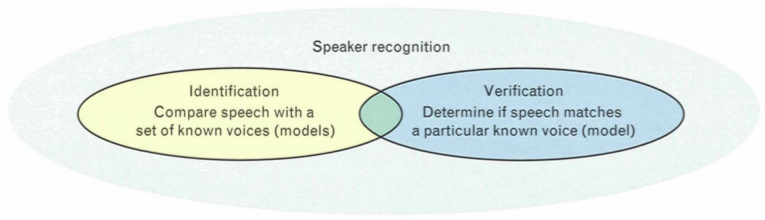
\includegraphics[width=0.75\textwidth]{speaker-recognition}
\end{figure}
\end{frame}

\begin{frame}
\frametitle{Dependência de texto}
\begin{description}
    \item[Dependente] Teste $\in$ Treinamento
    \pause
    \begin{itemize}
        \item Diversos graus de dependência
        \pause
        \item Teste $\not\in$ Treinamento $\implies$ Retreinamento
        \pause
    \end{itemize}
    \item[Independente] Teste $\neq$ Treinamento
    \pause
    \begin{itemize}
        \item Características não textuais
        \pause
        \item Presentes em diferentes sotaques e até \emph{gibberish}
    \end{itemize}
    \pause
    \item Este trabalho é focado em \textbf{reconhecimento de locutor independente de texto}
\end{description}
\end{frame}

\subsection{Modelos de Mistura Gaussiana}

\begin{frame}
\frametitle{Modelos de Mistura Gaussiana}
\begin{description}
    \item[GMM] Combinação de Gaussianas
    \pause
    \item[UBM] GMM gerado por diversas locuções de fundo
    \pause
    \item[AGMM] GMM adaptado a partir de um UBM
    \pause
    \item[FGMM] GMM utilizando Fractional Covariance Matrix (FCM)
\end{description}
\end{frame}

\subsection{Objetivos}

\begin{frame}
\frametitle{Objetivos}
\begin{description}
    \item Implementar sistemas de reconhecimento de locutor e analizar
    \pause
    \begin{itemize}
        \item Taxas de \textbf{sucesso} para identificação
        \pause
        \begin{itemize}
            \item Diferentes tamanhos de mistura ($M$)
            \pause
            \item Diferentes tamanhos de características
            \pause
        \end{itemize}
        \item Comparar identificação utilizando GMM e FGMM
        \pause
        \item Taxas de \textbf{falsa detecção} e \textbf{falsa rejeição} para verificação
        \pause
        \begin{itemize}
            \item Diferentes tamanhos de mistura ($M$)
            \pause
            \item Diferentes tamanhos de características
            \pause
        \end{itemize}
        \item Comparar verificação utilizando GMM e AGMM
    \end{itemize}
\end{description}
\end{frame}

\chapter{Speaker Recognition Systems}
\label{ch:speaker-recognition-systems}

%TODO remodelar, retirando tudo sobre Speaker IDENTIFICATION

The process of speaker recognition lies on the field of pattern classification, with the speaker's speech signal as input for a classifier. For an identification system, the classification is 1 to N (one speaker signal to be identified as belonging to one of the N enrolled speakers). The classification is considered correct if the identity assigned to the speaker matches his or her real identity. A verification system, on the other hand, is designed to determine if a claimed identity is true (user is classified as ``enrolled") or false (user is classified as ``imposter"). Differently from the speaker identification process, where the inputted speech is tested for all enrolled speakers and identified as the one with the highest score, in speaker verification only one speaker (the claimed identity) is tested. In order to perform a better comparison, a test against a model representing the other speakers is executed and the resulted score is compared with the score from the previous test, delivering a more reliable outcome.

\section{Utterance}

An \textbf{utterance} is a piece of speech produced by a speaker. It may be a word, a statement or any vocal sound. The terms \emph{utterance} and \emph{speech signal} sometimes are used interchangeably, but from herenow speech signal will be defined as an utterance recorded, digitalized and ready to be processed. An example is shown in \figureref{speech_signal}.

\begin{figure}[ht]
    \centering
    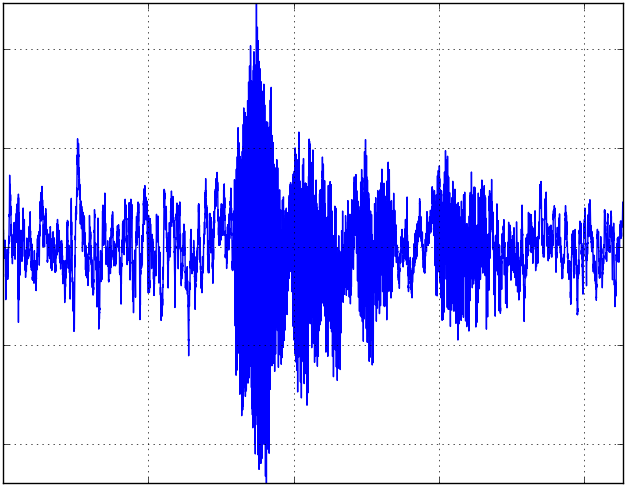
\includegraphics[width=\textwidth]{speech_signal}
    \caption{Speech signal from utterance ``karen livescu", \refbib{Woo, Park \& Hazen}{woo.park.hazen.2006}.}
    \label{fig:speech_signal}
\end{figure}

\section{Features}

The raw speech signal is unfit for use by an ASR system. For a correct processing, the representative features from the speaker's vocal tract are extracted, what reduces the number of variables the system needs to deal with (leading to a simpler implementation) and performs a better evaluation (prevents the curse of dimensionality). Due to the stationary properties of the speech signal when analyzed in a short period of time, it is divided in overlapping frames of small and predefined length, to avoid ``loss of significancy", \refbib{Davis \& Mermelstein}{davis.mermelstein.1980}, \refbib{Rabiner \& Schafer}{rabiner.schafer.2007}. This extraction is executed by the MFCC algorithm, explained in details in \chapterref{feature-extraction}.

\section{Speaker Identification}
\label{sec:speaker-identification}

Given the features $\dvec{X}$ extracted from a speech signal $\dvec{Y}$ spoken by an arbitrary speaker $\mathcal{S}$, the task of identify $\mathcal{S}$ as a particular $\mathcal{S}_i$ from $\dvec{\mathcal{S}}$ (set of enrolled users) is given by the following equation:

\begin{equation}
    \mathcal{S} \text{ is } \mathcal{S}_i \text{ if } i = \arg_j\max\postpdf{\boldsymbol{X}}{\mathcal{S}_j},
    \label{eq:classification_speaker_identification}
\end{equation}

\noindent for $j = 1, ..., S$ (with $S$ being the size of $\dvec{\mathcal{S}}$).

\subsection{Training}

The features extracted from speech signals are used to train models for the speakers. Each speaker $\mathcal{S}_i$ is represented by a model $\lambda_i$, generated using only the features belonging to the particular speaker.

\begin{figure}[ht]
    \centering
    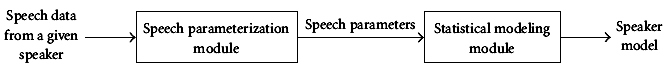
\includegraphics[width=\textwidth]{speaker-recognition-training}
    \caption{The statistical model of $\mathcal{S}$ is created from the speech signal $\dvec{Y}$, \refbib{Bimbot et. al.}{bimbot.et.al.2004}.}
    \label{fig:speaker-recognition-training}
\end{figure}

The SGMM, initially referenced in \sectionref{gmm}, is a perfect choice to model the $\lambda_i$'s.

\subsection{Test}

The system test is performed replacing $\mathcal{S}_i$ in \equationref{classification_speaker_identification} by the model $\lambda_i$, leading to

\begin{equation}
    \mathcal{S} \text{ is } \mathcal{S}_i \text{ if } i = \arg_j\max\postpdf{\boldsymbol{X}}{\lambda_j},
    \label{eq:speaker_identification}
\end{equation}

\begin{figure}[ht]
    \centering
    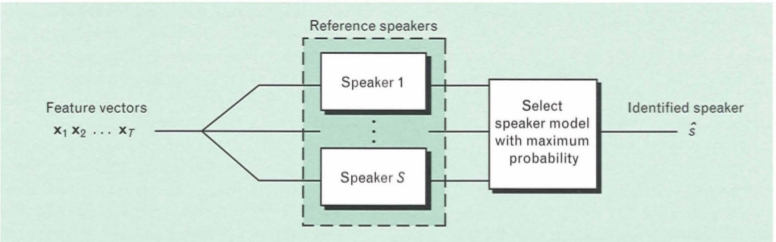
\includegraphics[width=\textwidth]{speaker-identification}
    \caption{Speaker identification test, \refbib{Reynolds}{reynolds.1995a}.}
    \label{fig:speaker_identification}
\end{figure}

\noindent where the model with higher probability has its identity assigned to $\mathcal{S}$. The main difficult this system presents is the fact that every $\dvec{X}$ must be tested with every $\mathcal{S}_i$ from $\dvec{\mathcal{S}}$, as seen in \figureref{speaker_identification}, what demands a high amount of time.

\section{Speaker Verification}
\label{sec:speaker-verification}

If a speaker $\mathcal{S}$ claims to be a particular user $\mathcal{S}_i$ from $\dvec{\mathcal{S}}$, the strength of this claim resides on how similar the features $\dvec{X}$ are to the features from $\mathcal{S}_i$ ``memorized" by the system. Then a simple equation

\begin{equation}
    \postpdf{\boldsymbol{X}}{\mathcal{S}_i} \verifytestB{\alpha}{\mathcal{S}}
    \label{eq:decision_speaker_verification}
\end{equation}

\noindent where $\alpha$ is an arbitrary coefficient, should be enough (considering all speakers equally probable). However, a subset of enrolled speakers may have vocal similarities or the features $\dvec{X}$ may be common to a large number of users, leading to a misclassification of an imposter as a registered speaker (a false detection). To reduce the error rate the system must decide not only if a speech signal came from the claimed speaker, but also if it came from a set composed of all other enrolled speakers and compare the likelihoods.

\subsection{Likelihood Ratio Test}

Given the vector of features $\dvec{X}$, and assuming it was produced by only one speaker, the detection\footnote{the terms verification and detection are used interchangeably} task can be restated as a basic test between two hypoteses, \refbib{Reynolds}{reynolds.1995b}:

\begin{description}\itemsep0pt
    \item $H_0$: $\dvec{X}$ is from the claimed speaker $\mathcal{S}_i$;
    \item $H_1$: $\dvec{X}$ is \underline{not} from the claimed speaker $\mathcal{S}_i$.
\end{description}

\noindent The optimum test to decide which hypotesis is valid is the \textbf{likelihood ratio test} between both likelihoods $\postpdf{\dvec{X}}{H_0}$ and $\postpdf{\dvec{X}}{H_1}$, \refbib{Reynolds, Quatieri \& Dunn}{reynolds.quatieri.dunn.2000},

\begin{equation}
    \frac{\postpdf{\dvec{X}}{H_0}}{\postpdf{\dvec{X}}{H_1}} \verifytestB{\theta}{H_0}
    \label{eq:likelihood-ratio-test}
\end{equation}

\noindent where the decision threshold for accepting or rejecting $H_0$ is $\theta$ (a low $\theta$ generates a more permissive system, while a high $\theta$, a more restrictive). Applying the logarithm, the behavior of the likelihood ratio is maintained and \equationref{likelihood-ratio-test} is replaced by the \textbf{log-likelihood ratio}

\begin{equation}
    \Lambda(\dvec{X}) = \log \postpdf{\dvec{X}}{H_0} - \log \postpdf{\dvec{X}}{H_1}.
    \label{eq:log-likelihood-ratio-test}
\end{equation}

\subsection{Training}

Once the features are extracted from the speech signal, they are used to train the models $\lambda_{hyp}$ and $\lambda_{\overline{hyp}}$ for $H_0$ and $H_1$, respectively. A high-level demonstration of the training of $\lambda_{hyp}$ (mathematical representation of $\mathcal{S}_i$) is shown in \figureref{speaker-recognition-training}:

Due to $\lambda_{hyp}$ be a model of $\mathcal{S}_i$, the features used for training (i.e., estimate $p(\dvec{X}|\lambda_{hyp})$) are extracted from speech signals produced by $\mathcal{S}_i$. The model $\lambda_{\overline{hyp}}$, however, is not well-defined. It should be composed of the features extracted from speech signals from all other speakers except $\mathcal{S}_i$, but creating a single $\lambda_{\overline{hyp}}$ for each speaker is complicated and with no expressive gain. Instead, what is normally done is use all speakers to generate a background model $\lambda_{bkg}$, \refbib{Reynolds}{reynolds.1997}, in which the weight of each $\mathcal{S}_i$ is minimized.

\subsection{Test}

As seen in \equationref{likelihood-ratio-test}, the decision process is based on a function \emph{Score}. Replacing each $H_j$ for its corresponding model, the likelihood of a $\lambda_j$ given $\dvec{X}$ can be written as

\begin{equation}
    p(\dvec{X}|\lambda_j) = \prod_{t=1}^T p(\dvec{x}_t|\lambda_j).
    \label{eq:likelihood-prod}
\end{equation}

\noindent Using the logarithm function, \equationref{likelihood-prod} becomes

\begin{equation}
    \log p(\dvec{X}|\lambda_j) = \frac{1}{T} \sum_{t=1}^T \log p(\dvec{x}_t|\lambda_j),
    \label{eq:log-likelihood-sum}
\end{equation}

\noindent where the term $\frac{1}{T}$ is used to normalize the log-likelihood to the duration of the speech signal. That said, the likelihood ratio given by \equationref{log-likelihood-ratio-test} becomes

\begin{equation}
    \Lambda(\dvec{X}) = \log p(\dvec{X}|\lambda_{hyp}) - \log p(\dvec{X}|\lambda_{bkg}),
    \label{eq:score_of_X}
\end{equation}

\noindent and the speaker is accepted if $\Lambda(\dvec{X}) \geq \theta$, for an arbitrary value\footnote{$\theta$ is loosely used here. The proper equation would be $\Lambda(\dvec{X}) \geq \log\theta$.} of $\theta$ (see \figureref{speaker-verification}).

\begin{figure}[ht]
    \centering
    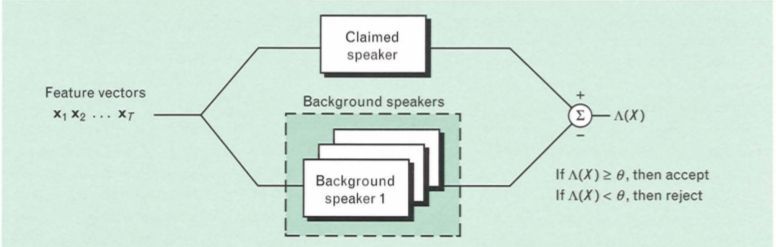
\includegraphics[width=\textwidth]{speaker-verification}
    \caption{Likelihood-ratio-based speaker verification system, \refbib{Bimbot et. al.}{bimbot.et.al.2004}.}
    \label{fig:speaker-verification}
\end{figure}

\section{Extração de Características}
\label{sec:feature-extraction}

\contentscurrent

\begin{frame}
\frametitle{Características Ideais}
\begin{itemize}
    \item Natural e frequente na fala
    \pause
    \item Facilmente mensurável
    \pause
    \item $\uparrow$ variação inter-locutor e $\downarrow$ variação intra-locutor
    \pause
    \item Constante no tempo e não afetável pela saúde
    \pause
    \item Robusta a ruído razoável e a transmissão
    \pause
    \item Difícil de ser produzido artificialmente
    \pause
    \item Não ser facilmente modificável pelo locutor
\end{itemize}
\end{frame}

\subsection{MFCC}

\begin{frame}
\frametitle{Mel-Frequency Cepstrum Coefficients}
\begin{description}
    \item Simula a função da \textbf{cóclea}
    \pause
    \item[Escala Mel] Logaritmica
    \pause
    \begin{itemize}
        \item $f_{mel} = 2595 \log_{10}(1 + \frac{f}{700})$
        \pause
    \end{itemize}
\end{description}

\begin{figure}[ht]
    \centering
    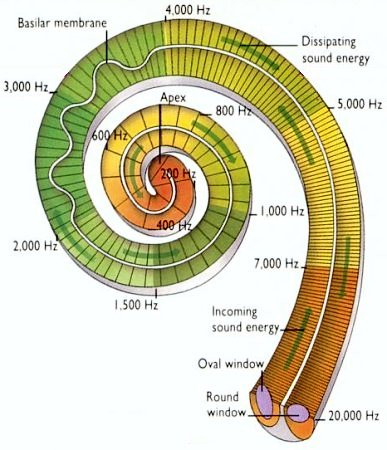
\includegraphics[width=0.35\textwidth]{cochlea}
\end{figure}
\end{frame}

\subsection{MFCC - Extração}

\begin{frame}
\frametitle{MFCC - Extração}
\begin{figure}[ht]
    \centering
    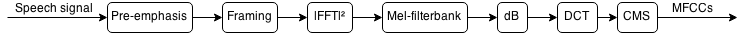
\includegraphics[width=0.75\textwidth]{mfcc-flow}
\end{figure}
\pause

\begin{description}
    \item[Pré-ênfase] \textbf{Realça} as altas frequências (opcional)
    \pause
    \begin{itemize}
        \item $s_{emph}[n] = s[n] - \alpha \cdot s[n - 1]$
        \pause
        \item $\alpha \in [0.95, 0.98]$
        \pause
    \end{itemize}
\end{description}
\begin{figure}[ht]
    \centering
    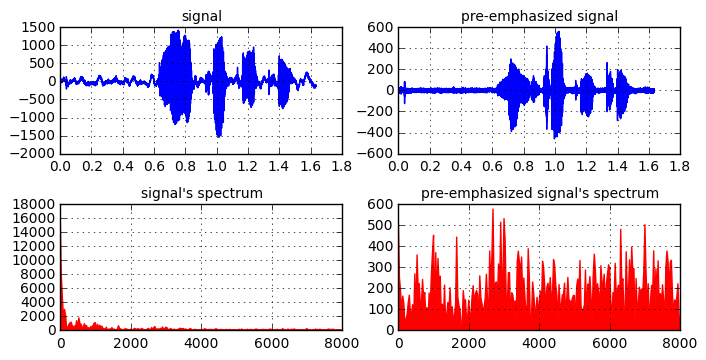
\includegraphics[width=0.75\textwidth]{preemphasis}
\end{figure}
\end{frame}

\subsection{MFCC - Extração}

\begin{frame}
\frametitle{MFCC - Extração}
\begin{figure}[ht]
    \centering
    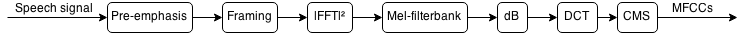
\includegraphics[width=0.75\textwidth]{mfcc-flow}
\end{figure}
\pause

\begin{description}
    \item[Janelamento] Divide o sinal em janelas \textbf{superpostas}
    \pause
    \begin{itemize}
        \item Largura de 20 milissegundos
        \pause
        \item Deslocamento de 10 milissegundos
        \pause
    \end{itemize}
\end{description}
\begin{figure}[ht]
    \centering
    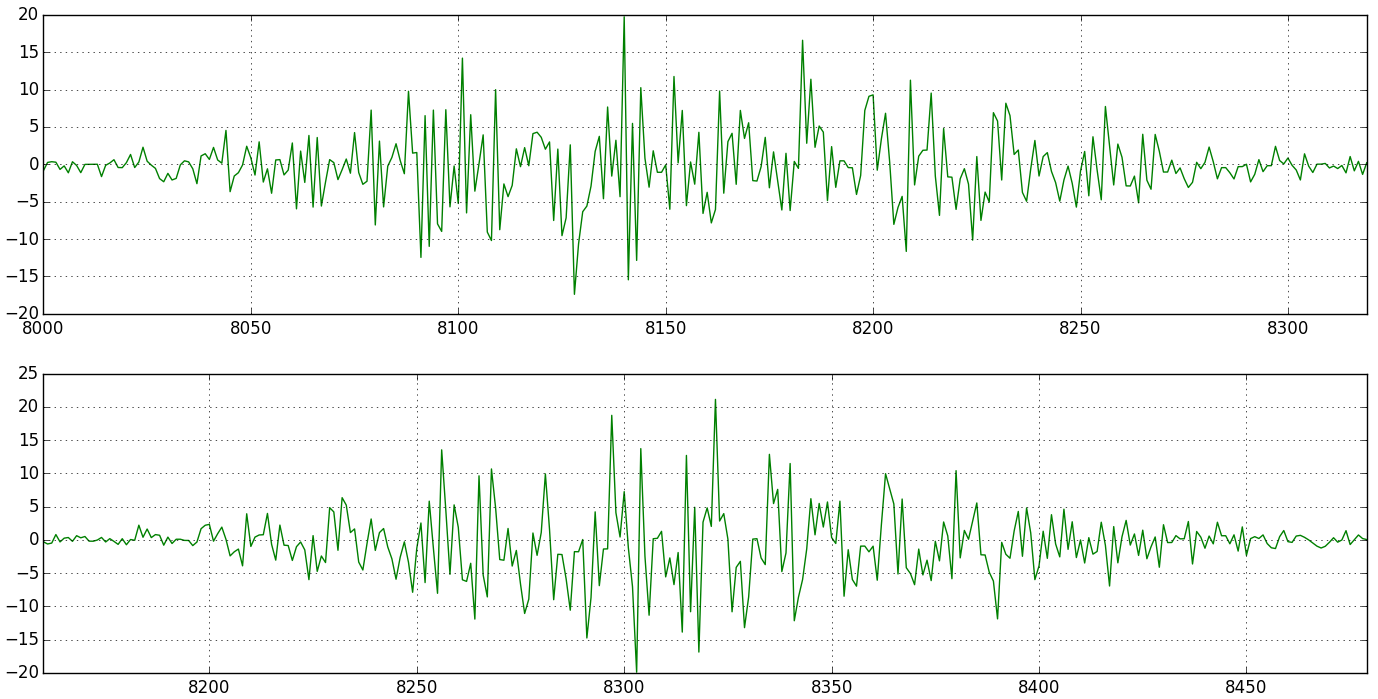
\includegraphics[width=0.75\textwidth]{framing}
\end{figure}
\end{frame}

\subsection{MFCC - Extração}

\begin{frame}
\frametitle{MFCC - Extração}
\begin{figure}[ht]
    \centering
    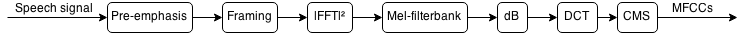
\includegraphics[width=0.75\textwidth]{mfcc-flow}
\end{figure}
\pause

\begin{description}
    \item[$|FFT|^2$] Calcula o \textbf{espectro de potência}
    \pause
\end{description}
\begin{figure}[ht]
    \centering
    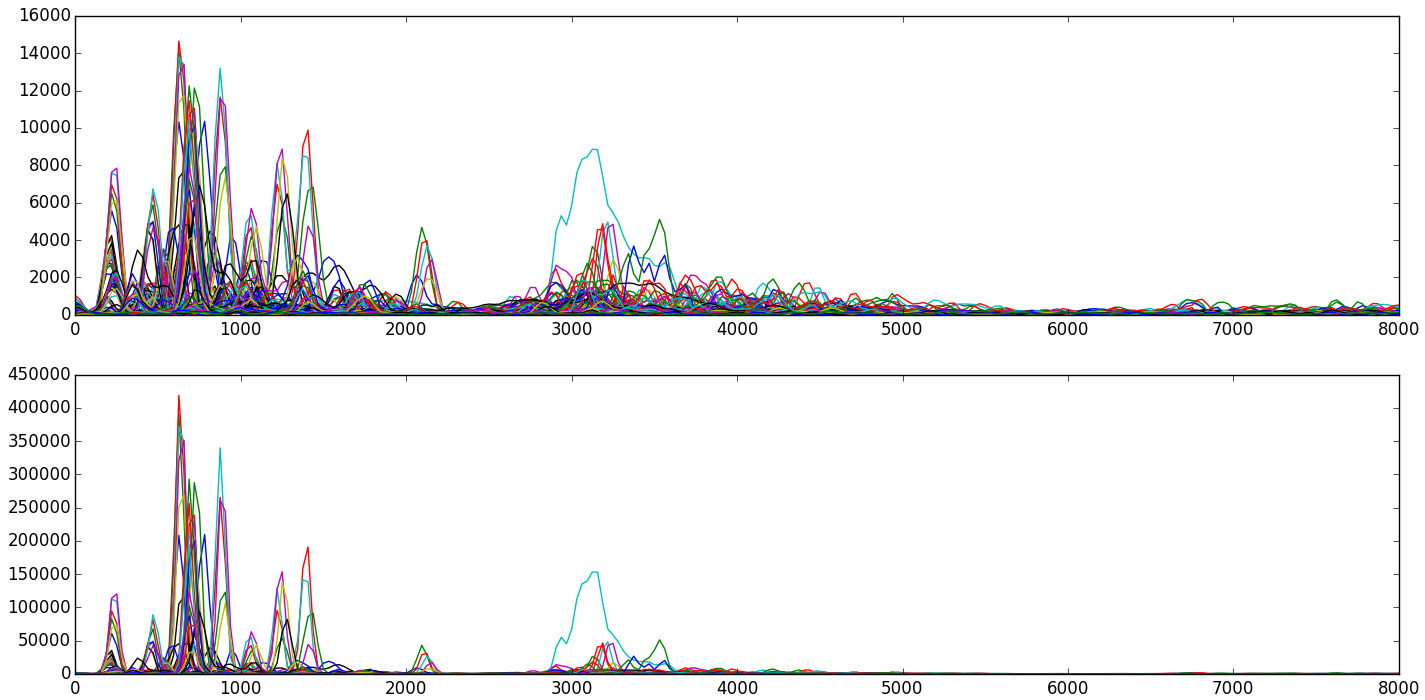
\includegraphics[width=0.6\textwidth]{fft}
\end{figure}
\end{frame}

\subsection{MFCC - Extração}

\begin{frame}
\frametitle{MFCC - Extração}
\begin{figure}[ht]
    \centering
    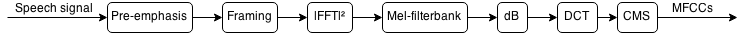
\includegraphics[width=0.75\textwidth]{mfcc-flow}
\end{figure}
\pause

\begin{description}
    \item[Filtros] Espectro em Hz $\implies$ espectro em \textbf{mels}
    \pause
\end{description}
\begin{figure}[ht]
    \centering
    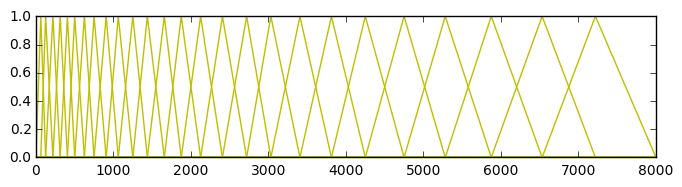
\includegraphics[width=0.75\textwidth]{filterbank}
\end{figure}
\end{frame}

\subsection{MFCC - Extração}

\begin{frame}
\frametitle{MFCC - Extração}
\begin{figure}[ht]
    \centering
    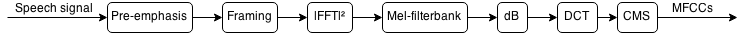
\includegraphics[width=0.75\textwidth]{mfcc-flow}
\end{figure}
\pause

\begin{description}
    \item[dB] Calcula a \textbf{sonoridade}
    \pause
\end{description}
\begin{figure}[ht]
    \centering
    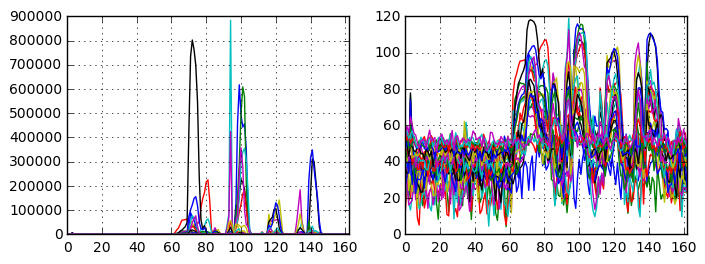
\includegraphics[width=0.75\textwidth]{features_and_featuresdB}
\end{figure}
\end{frame}

\subsection{MFCC - Extração}

\begin{frame}
\frametitle{MFCC - Extração}
\begin{figure}[ht]
    \centering
    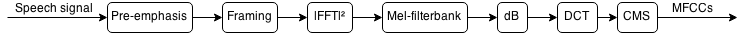
\includegraphics[width=0.75\textwidth]{mfcc-flow}
\end{figure}
\pause

\begin{description}
    \item[DCT] Coeficientes espectrais $\implies$ coeficientes \textbf{cepstrais}
    \pause
    \begin{itemize}
        \item $c_n = \sum_{k=1}^K S_k\cdot\cos\left[n\left(k - \frac{1}{2}\right)\frac{\pi}{K}\right], n = 1, 2, ..., L$
        \pause
    \end{itemize}
\end{description}
\begin{figure}[ht]
    \centering
    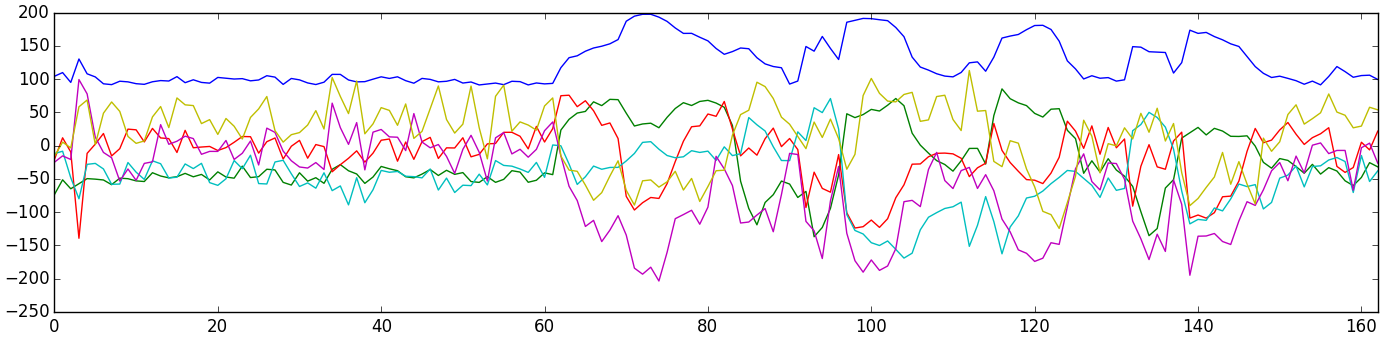
\includegraphics[width=0.7\textwidth]{mfcc}
\end{figure}
\begin{figure}[ht]
    \centering
    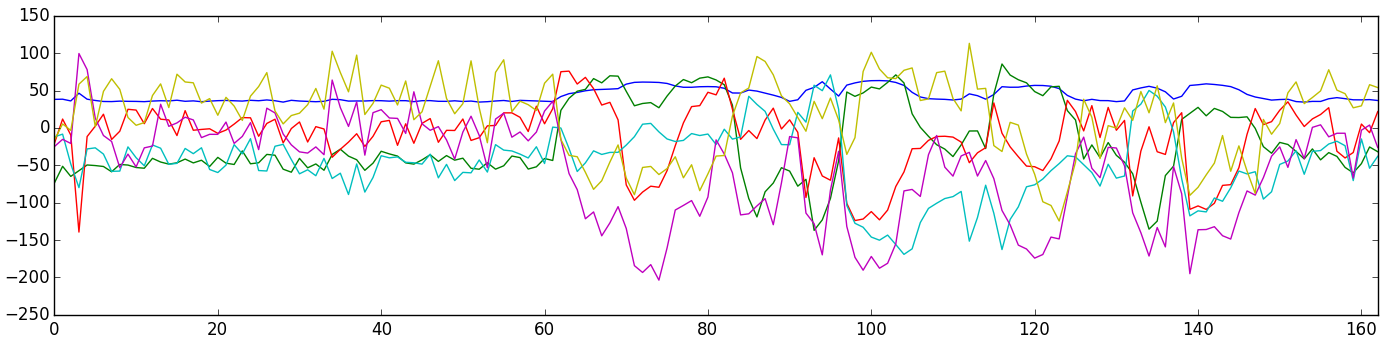
\includegraphics[width=0.7\textwidth]{mfcc_energy_appended}
\end{figure}
\end{frame}

\subsection{MFCC - Extração}

\begin{frame}
\frametitle{MFCC - Extração}
\begin{figure}[ht]
    \centering
    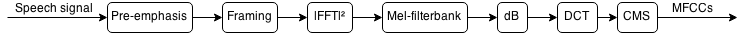
\includegraphics[width=0.75\textwidth]{mfcc-flow}
\end{figure}
\pause

\begin{description}
    \item[CMS] \textbf{Normaliza} os MFCCs para reduzir perturbações
    \pause
    \begin{itemize}
        \item $c_n = c_n - \frac{1}{T} \sum_{t=1}^T c_{n,t}$
        \pause
    \end{itemize}
\end{description}
\begin{figure}[ht]
    \centering
    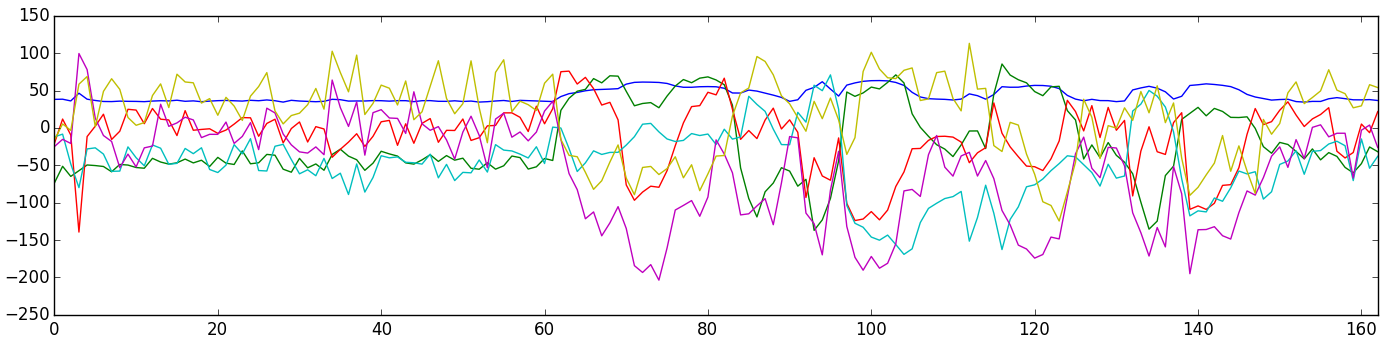
\includegraphics[width=0.7\textwidth]{mfcc_energy_appended}
\end{figure}
\begin{figure}[ht]
    \centering
    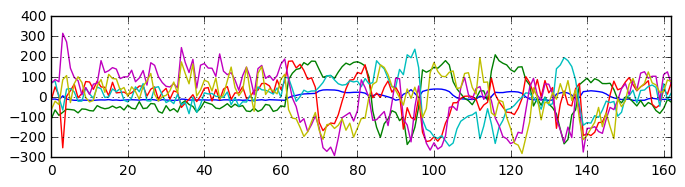
\includegraphics[width=0.7\textwidth]{mfcc_energy_appended_cms}
\end{figure}
\end{frame}

\subsection{MFCC - Extração}

\begin{frame}
\frametitle{MFCC - Extração}
\begin{figure}[ht]
    \centering
    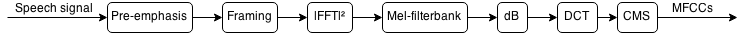
\includegraphics[width=0.75\textwidth]{mfcc-flow}
\end{figure}
\pause

\begin{description}
    \item[$\dvec{\Delta}$s] Novos $c_n$ \textbf{derivados} dos antigos $c_n$ (opcional)
    \pause
    \begin{itemize}
        \item $\Delta_t = \frac{\sum_{n=1}^N n(c_{t+n} - c_{t-n})}{2\sum_{n=1}^N n^2}$
        \pause
    \end{itemize}
\end{description}
\begin{figure}[ht]
    \centering
    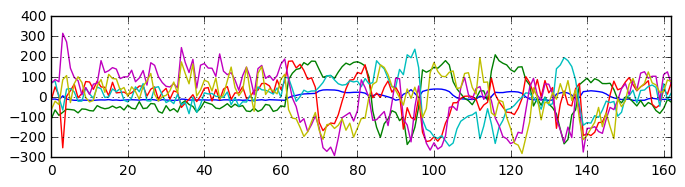
\includegraphics[width=0.7\textwidth]{mfcc_energy_appended_cms}
\end{figure}
\begin{figure}[ht]
    \centering
    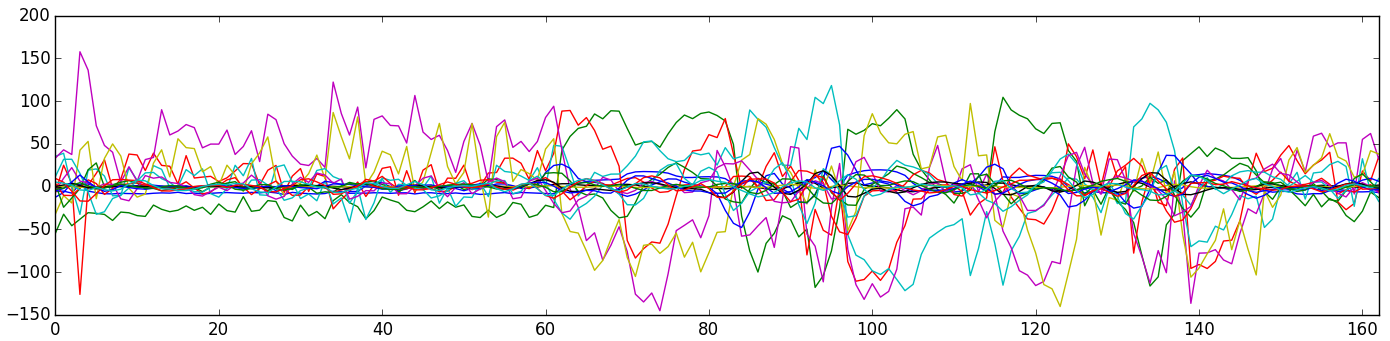
\includegraphics[width=0.7\textwidth]{mfcc_energy_appended_cms_delta_order_2}
\end{figure}
\end{frame}

\chapter{Gaussian Mixture Models}
\label{ch:gmm}

\chapterref{speaker-recognition-systems} briefly discussed the use of models $\lambda_j$ to perform an identification process and models $\lambda_{C}$ and $\lambda_{bkg}$ for a claimed speaker and for a background composed of all enrolled speakers, respectively, to a verification process. As the features from the speech signal have unknown values until the moment of extraction, it is reasonable to model the ASR system to work with random values.

For all sorts of probability distributions, the Gaussian (or normal) is the one that best describes the behavior of a random variable of unknown distribution, as demonstrated by the central limit theorem. Its equation for a D-dimensional space is

\begin{equation}
    \pdf{\dvec{x}} = \postpdf{\dvec{x}}{\dvec{\mu},\dvec{\Sigma}} = \dgaussian{x}{\mu}{\Sigma},
    \label{eq:gaussian}
\end{equation}

\noindent where $\dvec{x}$ is a $D$-dimensional input vector, $\dvec{\mu}$ is a $D$-dimensional vector of means, $\dvec{\Sigma}$ is a $D \times D$ matrix of covariances, $\dvec{|\Sigma|}$ is the determinant of $\dvec{\Sigma}$, and $(\dvec{x} - \dvec{\mu})'$ is the transposed of the colum-matrix $(\dvec{x} - \dvec{\mu})$.

\section{Definition}
\label{sec:gmm-definition}

For the general case, a single Gaussian distribution does not provide the most accurate representation. This issue is reduced using a linear combination of $\pdf{\dvec{x}}$'s to model the ASR system, estimating the one that best represents the training data. This combination is named Gaussian Mixture Model (GMM), first used for speaker recognition in \refbib{Reynolds}{reynolds.1992}, and given by

\begin{equation}
    \postpdf{\dvec{x}}{\lambda} = \sum_{i=1}^M w_i\postpdfi{\dvec{x}}{\dvec{\mu}_i, \dvec{\Sigma}_i} = \sum_{i=1}^M w_i\pdfi{\dvec{x}},
    \label{eq:gaussian_mixture}
\end{equation}

\noindent where $M$ is the size of the distribution used, $\sum_{i=1}^M w_i = 1$, and $\lambda = \{(w_i, \dvec{\mu}_i, \dvec{\Sigma}_i)\}$ is the model representation, for $i = 1, ..., M$. Each Gaussian in each model has its own covariance matrix (nodal covariance). Applying \equationref{gaussian} to \equationref{gaussian_mixture}, the likelihood for the GMM is

\begin{equation}
    \postpdf{\dvec{x}}{\lambda} = \dgaussianmixture.
    \label{eq:likelihood_gmm}
\end{equation}

The reason to model a speaker $\mathcal{S}$ using a GMM is to achieve a $\lambda$ that maximizes the likelihood when applied to features $\dvec{x}$ extracted from a speech signal produced by $\mathcal{S}$. This value is found by a Maximum Likelihood Estimation (MLE) algorithm. For a sequence of T training vectors $\boldsymbol{X} = \{\dvec{x}_t\}$, the GMM's likelihood can be written as

\begin{equation}
    \postpdf{\boldsymbol{X}}{\lambda} = \prod_{t=1}^T \postpdf{\dvec{x}_t}{\lambda}.
    \label{eq:likelihood_gmm_mle}
\end{equation}

\noindent Unfortunately, this expression is a nonlinear function of the parameter $\lambda$ and direct maximization is not possible, \refbib{Reynolds}{reynolds.1995c}, leading to estimate $\postpdf{\dvec{x}}{\lambda}$ iteratively using the Expectation-Maximization (EM) algorithm.

In this report, the GMM that models a single speaker will be reffered to as Single Speaker Gaussian Mixture Model (SSGMM), as initially cited in \sectionref{gmm}.

\section{Expectation-Maximization}
\label{sec:em}

The idea of the EM algorithm is to estimate a new model $\lambda^{(k+1)}$ from a previous model $\lambda^{(k)}$, that obeys $\postpdf{\boldsymbol{X}}{\lambda^{(k+1)}} \geq \postpdf{\boldsymbol{X}}{\lambda^{(k)}}$, better representing the training data at each iteration until some convergence threshold is reached. The algorithm is composed of 2 steps, an expectation of the \emph{a posteriori} probabilities for each distribution $i$, and a maximization step, when the parameters $w_i$, $\dvec{\mu}_i$ and $\dvec{\Sigma}_i$ are updated. The following description of the steps uses a $\lambda$ with \textbf{diagonal}\footnote{As stated in \refbib{Reynolds et. al.}{reynolds.quatieri.dunn.2000}, diagonal covariance matrix GMMs outperform and are more computationally efficient than full covariance matrix GMMs. Also, the density modeling of an $M$-th order full covariance matrix GMM can equally well be achieved using a larger order diagonal covariance.} $\dvec{\Sigma}_i$ (i.e., change the $D \times D$ matrix $\dvec{\Sigma}_i$ for a $D$-dimensional vector $\dvec{\sigma}_i^2$ of variances).

\subsubsection*{E-Step}

The \textbf{expectation step} consists of estimating the \emph{a posteriori} probabilities $\postprob{i}{\dvec{x}_t, \lambda}$ for each distribution $i$ and each feature vector $\dvec{x}_t$, defined as

\begin{equation}
    \postprob{i}{\dvec{x}_t, \lambda} = \postprob{i}{\dvec{x}_t} = \frac{w_i p_i(\dvec{x}_t)}{\sum_{k=1}^M w_k p_k(\dvec{x}_t)}.
    \label{eq:e-step-posterior}
\end{equation}

\noindent The $\lambda$ present in \equationref{e-step-posterior} is the previously cited $\lambda^{(k)}$ for the current iteration.

\subsubsection*{M-Step}

In the \textbf{maximization step} the model is updated by recalculation of the parameters $w_i, \dvec{\mu}_i$ and $\dvec{\Sigma}_i$, and the algorithm guarantees that each new $\lambda^{(k+1)}$ represents the training data better than the previous ones. From \refbib{Reynolds}{reynolds.1995c}, the updates of $w_i$, $\dvec{\mu}_i$ and $\dvec{\sigma}_i^2$ are given by the equations below.

\noindent\\\textbf{Weights:}

\begin{equation}
    \overline{w}_i = \frac{1}{T} \sum_{t=1}^T \postprob{i}{\dvec{x}_t, \lambda},
    \label{eq:m-step-weight}
\end{equation}

\noindent\\\textbf{Means:}

\begin{equation}
    \overline{\dvec{\mu}}_i = \frac{\sum_{t=1}^T \postprob{i}{\dvec{x}_t, \lambda} \dvec{x}_t}{\sum_{t=1}^T \postprob{i}{\dvec{x}_t, \lambda}},
    \label{eq:m-step-means}
\end{equation}

\noindent\textbf{Variances:}

\begin{equation}
    \overline{\dvec{\sigma}}_i^2 = \frac{\sum_{t=1}^T \postprob{i}{\dvec{x}_t, \lambda} \dvec{x}_t^2}{\sum_{t=1}^T \postprob{i}{\dvec{x}_t, \lambda}} - \overline{\dvec{\mu}}_i^2,
    \label{eq:m-step-variances}
\end{equation}

\noindent\\ where $\lambda^{(k+1)} = \{(\overline{w}_i, \overline{\dvec{\mu}}_i, \overline{\dvec{\sigma}}_i^2)\}$, for $i = 1, \dots, M$, and $\lambda^{k} = \lambda^{(k+1)}$ in the next iteration. This algorithm trains the GMMs used in the ASR systems shown in sections \sectionrefcomp{speaker-identification} and \sectionrefcomp{speaker-verification} and previously described in \sectionref{gmm-definition}.

\begin{algorithm}
\label{em-algorithm}
\begin{algorithmic}[1]
\Procedure{Expectation\textendash Maximization}{$\lambda, \boldsymbol{X}, threshold$}
\State $\lambda^k = \lambda$
\State $\lambda^{(k+1)} =$ M-Step($\lambda^k, \boldsymbol{X})$
\State \textbf{if} $\postpdf{\boldsymbol{X}}{\lambda^{(k+1)}} - \postpdf{\boldsymbol{X}}{\lambda^{(k)}} \leq threshold \implies$ \textbf{goto} line $7$
\State$\lambda^k = \lambda^{(k+1)}$
\State \textbf{goto} line $3$
\EndProcedure
\end{algorithmic}
\end{algorithm}

\noindent The pseudo code above describes the EM algorithm. The \emph{E-Step} is not shown, but is used inside the \emph{M-Step}. Obviously, in an implementation the \emph{E-Step} is calculated once for each iteration. \figureref{em_algorithm} shows $\lambda$'s Gaussians before and after the EM algorithm.

\begin{figure}[ht]
    \centering
    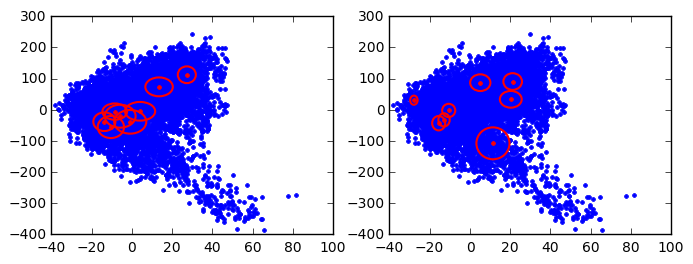
\includegraphics[width=\textwidth]{chapters/gmm/em_algorithm}
    \caption{Gaussians before (left), partitioned using a single iteration k-means, and after (right) the EM algorithm. Only the first deviation is shown.}
    \label{fig:em_algorithm}
\end{figure}

\section{Universal Background Model}
\label{sec:ubm}

An Universal Background Model (UBM) is a GMM composed of features from all enrolled speakers and used in speaker verification. The idea is to generate a model $\lambda_{bkg}$ where common characteristics present in this group are well represented. Then, a speech mostly composed of these characteristics is more difficult to succeed the likelihood ratio test, due to the low score produced by \equationref{score_of_X}.

There are many configurations for an UBM, however, as seen in \refbib{Reynolds et. al.}{reynolds.quatieri.dunn.2000}, male and female speakers present distinct vocal traits and are better represented when trained separately. Also, female voices have more intrasimilarities than males, leading to more distinct male configurations. The $M$-th order UBM in this study is created merging trained male and female models of order $M/2$ (see \figureref{ubm-diagram}).

\begin{figure}[ht]
    \centering
    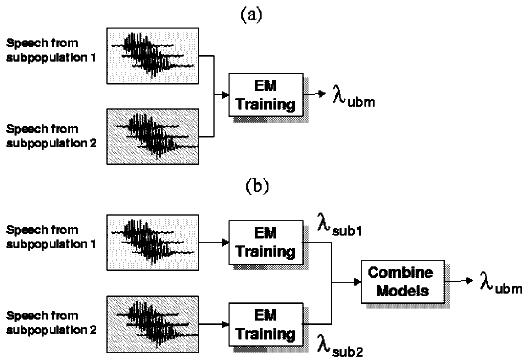
\includegraphics[width=0.55\textwidth]{chapters/gmm/ubm-diagram}
    \caption{UBM with gender trained (a) together and (b) separately and combined, \refbib{Reynolds et. al.}{reynolds.quatieri.dunn.2000}.}
    \label{fig:ubm-diagram}
\end{figure}

As shown in \sectionref{speaker-verification}, the likelihood ratio test is performed using the models $\lambda_{C}$ and $\lambda_{bkg}$. The default ASR system is a SSGMM-UBM system, turning \equationref{score_of_X} in

\begin{equation}
    \Lambda(\boldsymbol{X}) = \log p(\boldsymbol{X}|\lambda_{SSGMM}) - \log p(\boldsymbol{X}|\lambda_{UBM}).
    \label{eq:score_of_X_ssgmm_ubm}
\end{equation}

\section{Adapted Gaussian Mixture Model}
\label{sec:adapted-gmm}

As seen in \chapterref{speaker-recognition-systems} and in the previous sections, to perform the verification process a GMM for the claimed speaker and an UBM must be trained. Verify the entire corpus demands the training of SSGMMs for all enrolled speakers, a highly costly action in time. An effective alternative is to take advantage of the well-trained $M$-th order UBM, since the SSGMMs and the UBM must have the same order to use \equationref{score_of_X_ssgmm_ubm}, and adapt its parameters to generate a new SSGMM for a speaker, \refbib{Brown et. al.}{brown.lee.spohrer.1983}. This technique provides a faster modeling than in the SSGMM-UBM system (there is no loop of indefinite time such as in the EM algorithm) and tighter coupling between the speaker’s model and the UBM, \refbib{Reynolds et. al.}{reynolds.quatieri.dunn.2000}. The resultant GMM is named Single Speaker Adapted Gaussian Mixture Model (SSAGMM). Refactoring \equationref{score_of_X_ssgmm_ubm}, the log-likelihood ratio test for Adapted Gaussian Mixture Model (AGMM) is

\begin{equation}
    \Lambda(\boldsymbol{X}) = \log p(\boldsymbol{X}|\lambda_{SSAGMM}) - \log p(\boldsymbol{X}|\lambda_{UBM}).
    \label{eq:score_of_X_ssagmm_ubm}
\end{equation}

The Bayesian adaptation\footnote{Also known as \textbf{maximum a posteriori} (MAP) estimation.} reestimates the Gaussians from the UBM using features from the desired speaker only. If a Gaussian represents the new data better than the old data, the change is relevant.

The adaptation process is composed of two steps. The first is an expectation step, similar to the one in the EM algorithm. Using $\postprob{i}{\dvec{x}_t}$ from \equationref{e-step-posterior}, it is possible to compute the sufficient statistics for the weight, mean, and variance parameters:\footnote{$\dvec{x}^2$ is shorthand for diag($\dvec{x}\dvec{x}'$).}

\begin{equation}
    n_i = \sum_{t=1}^{T} \postprob{i}{\dvec{x}_t}
    \label{eq:n_i}
\end{equation}

\begin{equation}
    E_i(\dvec{x}) = \frac{1}{n_i} \sum_{t=1}^{T} \postprob{i}{\dvec{x}_t} \dvec{x}_t
    \label{eq:E_x}
\end{equation}

\begin{equation}
    E_i(\dvec{x}^2) = \frac{1}{n_i} \sum_{t=1}^{T} \postprob{i}{\dvec{x}_t} \dvec{x}_t^2
    \label{eq:E_x2}
\end{equation}

Finally, these new sufficient statistics from the training data are used to update the old UBM sufficient statistics and adapt the parameters for mixture $i$ with the equations taken from \refbib{Reynolds et. al.}{reynolds.quatieri.dunn.2000}:

\begin{equation}
    \hat{w_i} = [\alpha_i n_i / T + (1 - \alpha_i)w_i]\gamma
    \label{eq:adapted_weight}
\end{equation}

\begin{equation}
    \hat{\dvec{\mu}_i} = \alpha_i E_i(\dvec{x}) + (1 - \alpha_i)\dvec{\mu}_i
    \label{eq:adapted_means}
\end{equation}

\begin{equation}
    \hat{\dvec{\sigma}_i}^2 = \alpha_i E_i(\dvec{x}^2) + (1 - \alpha_i)(\dvec{\sigma}_i^2 + \dvec{\mu}_i^2) - \hat{\dvec{\mu}_i}^2.
    \label{eq:adapted_variances}
\end{equation}

\noindent The scale factor $\gamma$ normalizes the weights. \noindent The adaptation coefficient controlling the balance between old and new estimates is $\alpha_i$, given by\footnote{The equation for $\alpha_i$ is a simplification used in \refbib{Reynolds et. al.}{reynolds.quatieri.dunn.2000} with negligible loss. For the original equations for $\alpha_i^\rho$, $\rho = \{w, \dvec{\mu}, \dvec{\sigma}^2\}$, visit the referenced paper.}

\begin{equation}
    \alpha_i = \frac{n_i}{n_i + r},
    \label{eq:alpha_i}
\end{equation}

\noindent where $r$ is a fixed relevance factor. If a mixture component has a low probabilistic count $n_i$, then $\alpha_i \to 0$ causing the deemphasis of the new (potentially undertrained) parameters and the emphasis of the old (better trained) parameters. For mixture components with high probabilistic counts, $\alpha_i \to 1$, causing the use of the new speaker-dependent parameters. The relevance factor $r$ controls the strength of the new data in the adaptation process. Higher values of $r$ demand that more data be observed in a mixture before new parameters begin replacing olds.

\begin{figure}[ht]
    \centering
    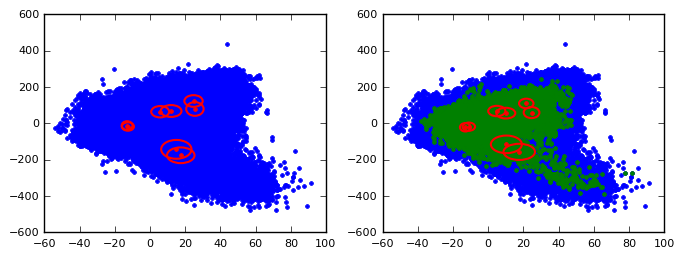
\includegraphics[width=\textwidth]{chapters/gmm/adapted_wmv}
    \caption{UBM trained (left) and weights, means and variances adapted for a female speaker (right) with $r = 16$. The blue dots are the background features and the green the speaker's. Only the first deviation is shown.}
    \label{fig:adapted_wmv}
\end{figure}

\section{Fractional Gaussian Mixture Model}
\label{sec:frac-gmm}

\refbib{Gao et. al.}{gao.zhou.pu.2013} uses the definition and applications of fractional moments to propose a new technique applying Fractional Covariance Matrix (FCM) in Principal Component Analysis (PCA) and Two-Dimensional Principal Component Analysis (2D-PCA), named Fractional Principal Component Analysis (FPCA) and Two-Dimensional Fractional Principal Component Analysis (2D-FPCA), respectively. The experiments are executed on two face image databases (ORL and Yale), using

\begin{equation}
    \sigma^2 = E[(X^r - \mu^r)^2],
    \label{eq:frac-variance}
\end{equation}

\noindent where $E$ is the expected value and $r$ is a real number, and show superior performance when choosing different values for $r$ between 0 and 1. A value of 1 for $r$ reduces \equationref{frac-variance} to the usual variance. As demonstrated in \refbib{Gao et. al.}{gao.zhou.pu.2013}, FPCA and 2D-FPCA deliver better projections than the usual PCA and 2D-PCA, respectively, making natural to extrapolate this idea for other types of signals and parametrizations.

The technique described in this section, named Fractional Gaussian Mixture Model (FGMM), also uses the theory of FCM to calculate matrices of covariances. As the matrices are diagonal, \equationref{frac-variance} is sufficient, changing \equationref{m-step-variances} to

\begin{equation}
    \overline{\dvec{\sigma}}_i^2 = \frac{\sum_{t=1}^T \postprob{i}{\dvec{x}_t, \lambda} (\dvec{x}_t^r - \overline{\dvec{\mu}}_i^r)^2}{\sum_{t=1}^T \postprob{i}{\dvec{x}_t, \lambda}}.
    \label{eq:m-step-frac-variances}
\end{equation}

\noindent One problem the FCM generates when applied to MFCCs is the emergence of complex numbers. A practical solution is to shift the MFCCs (see \figureref{mfcc-shifted}), turning all values in positive numbers and their minimums equal to 1:

\begin{equation}
    c_n = c_n + (1 - \min_t c_{n,t}).
    \label{eq:mfccs-shift-up}
\end{equation}

\noindent The distances in each dimension between points remain the same, maintaining the usual variances unchanged. \equationref{mfccs-shift-up} works correctly for GMMs with diagonal covariance matrices, due to the independence of each variable to the others. This ensures the correct uses of \equationref{frac-variance} to calculate the initial fractional variances and of \equationref{m-step-frac-variances} to train the models.

\begin{figure}[ht]
    \centering
    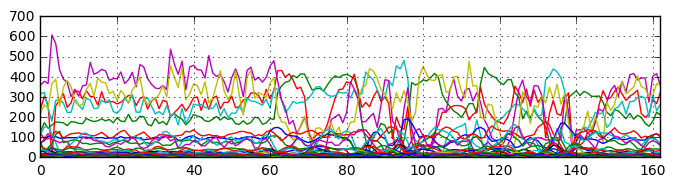
\includegraphics[width=\textwidth]{chapters/gmm/mfcc_energy_appended_cms_delta_order_2_shifted}
    \caption{MFCCs from \figureref{mfcc_energy_appended_cms_delta_order_2} shifted up. The minimum value for each feature is 1.}
    \label{fig:mfcc-shifted}
\end{figure}

\noindent After the variances are calculated, the means are shifted,

\begin{equation}
    \mu_n = \mu_n - (1 - \min_t c_{n,t}),
    \label{eq:means-shift-down}
\end{equation}

\noindent returning to their supposed ``original" values. This procedure avoids having to shift every vector of features, be it in the training or in the test sections, and is a practical solution to circumvent the problem.

\begin{figure}[ht]
    \centering
    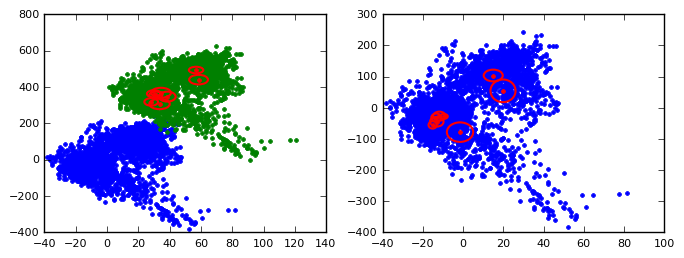
\includegraphics[width=\textwidth]{chapters/gmm/em_algorithm_r095}
    \caption{Features before (left), partitioned using k-means, and after (right) the EM algorithm. All variances (before and after EM) were calculated using FCM with $r = 0.95$. The blue points are the original features, while the greens are the shifted. Only the first deviation is shown.}
    \label{fig:frac-em_algorithm}
\end{figure}

The choice of shift all features to 1 is mostly based in common sense. To avoid non-negative values, just shift to 0 would be sufficient. However, when $r \to 0$, the results for $X^r$ and $\mu^r$ would fall in the indefinition $0^0$, due to approximations of floating points in numeric computation. Also, for values greater than or equal to 1, the exponentiation is a monotonic function.

\section{Experimentos}
\label{sec:experiments}

\contentscurrent

\subsection{Implementação}

\begin{frame}
\frametitle{Corpus}
\begin{description}
    \item[Base] MIT Mobile Device Speaker Verification Corpus
    \pause
    \item 54 locuções/locutor em 3 níveis de ruído
    \pause
    \begin{description}
        \item[Baixo] Escritório calmo
        \pause
        \item[Médio] Saguão de edfício
        \pause
        \item[Alto] Cruzamento movimentado
        \pause
    \end{description}
    \item 3 sessões distintas
    \begin{description}
        \item[Enroll 1] Treinamento dos modelos
        \pause
        \item[Enroll 2] Teste de detecção
        \pause
        \item[Imposter] Teste de rejeição
        \pause
    \end{description}
\end{description}

\begin{table}[h]
    \centering
    \begin{tabular}{|l|c|c|c|c|}
    \hline
    \multicolumn{1}{|c|}{{\bf Session}} & {\bf Training} & {\bf Test} & {\bf \#female} & {\bf \#male} \\ \hline
    Enroll 1 & {\bf X} & {\bf } & 22 & 26 \\ \hline
    Enroll 2 & {\bf } & {\bf X} & 22 & 26 \\ \hline
    Imposter & {\bf } & {\bf X} & 17 & 23 \\ \hline
    \end{tabular}
\end{table}
\end{frame}

\begin{frame}
\frametitle{Codificação}
\begin{description}
    \item[Linguagem] Python 3.4.3
    \pause
    \item[Frameworks] NumPy 1.8.1, SciPy 0.14.0, Matplotlib 1.4
    \pause
    \item[Parâmetros] A implementação utilizou
    \pause
    \begin{itemize}
        \item \# filtros = 26
        \pause
        \item \# coefficientes = 19
        \pause
        \item $\Delta$s de ordem 0, 1 e 2, com $K = 2$
        \pause
        \item Energy appending e CMS
        \pause
        \item $r = 16$ para AGMM
        \pause
        \item $threshold = 10^{-3}$ no EM
        \pause
        \item $M = 8, 16, 32, 64, 128$
    \end{itemize}
\end{description}
\end{frame}

\begin{frame}
\frametitle{Percalços}
\begin{description}\itemsep6pt
    \item[Inicialização] Em 2 passos
    \pause
    \begin{itemize}
        \item Escolha de médias aleatórias
        \pause
        \item \emph{k-means} $\implies$ Novas médias + pesos e variâncias
        \pause
    \end{itemize}
    \item[Variâncias] Podem reduzir significativamente
    \pause
    \begin{itemize}\itemsep4pt
        \item $\sigma_{min}^2 = 0.01$
        \pause
        \item $\sigma^2 < \sigma_{min}^2 \implies \sigma^2 \gets \sigma_{min}^2$
        \pause
    \end{itemize}
    \item[$\overline{Monotonic}$] FGMM viola $\log\postpdf{\dvec{X}}{\lambda^{(k+1)}} \geq \log\postpdf{\dvec{X}}{\lambda^{k}}$
    \begin{itemize}\itemsep4pt
        \item $|1 - r| \implies \downarrow$ estimação
    \end{itemize}
\end{description}
\end{frame}

\subsection{Experimentos}

\begin{frame}
\frametitle{Identificação}
\end{frame}

\chapter{Conclusion}
\label{ch:conclusion}

TODO escrever a conclusão após terminar tudo (antes do abstract)


%BACKMATTER

\appendix
\chapter{Results for Identification using SSFGMM}
\label{apx:results-identify-ssfgmm}

\section{Table and curves for $r = 0.95$}

\begin{table}[h]
    \centering
    \begin{tabular}{|c|c|M{2cm}|M{2cm}|M{2cm}|M{2cm}|}
    \hline
    $\boldsymbol{\Delta}$ & \bf{M} & \bf{Office} & \bf{Hallway} & \bf{Intersection} & \bf{All} \\
    \hline
    \hline
     & \bf{8} & 38.70 & 44.41 & 32.37 & 50.50 \\
    \cline{2-6}
     & \bf{16} & 41.63 & 46.37 & 32.56 & 62.35 \\
    \cline{2-6}
    \multirow{5}{*}\bf{\textbf 0} & \bf{32} & 47.72 & 48.53 & 37.46 & 68.06 \\
    \cline{2-6}
     & \bf{64} & 43.75 & 50.31 & 37.27 & 72.80 \\
    \cline{2-6}
     & \bf{128} & 38.62 & 42.75 & 31.06 & 72.15 \\
    \hline
    \hline
     & \bf{8} & 33.37 & 31.67 & 26.35 & 44.87 \\
    \cline{2-6}
     & \bf{16} & 41.13 & 42.32 & 26.62 & 54.71 \\
    \cline{2-6}
    \multirow{5}{*}\bf{\textbf 1} & \bf{32} & 44.95 & 47.92 & 30.29 & 64.47 \\
    \cline{2-6}
     & \bf{64} & 43.13 & 43.36 & 31.64 & 70.95 \\
    \cline{2-6}
     & \bf{128} & 33.14 & 37.15 & 21.10 & 73.84 \\
    \hline
    \hline
     & \bf{8} & 32.21 & 33.49 & 26.66 & 43.02 \\
    \cline{2-6}
     & \bf{16} & 41.09 & 42.40 & 31.10 & 54.67 \\
    \cline{2-6}
    \multirow{5}{*}\bf{\textbf 2} & \bf{32} & 46.33 & 44.14 & 31.75 & 66.78 \\
    \cline{2-6}
     & \bf{64} & 40.93 & 43.60 & 33.53 & 72.72 \\
    \cline{2-6}
     & \bf{128} & 39.16 & 37.89 & 23.26 & 73.53 \\
    \hline
    \end{tabular}
    \caption{Identification rates for enrolled speakers with $r = 0.95$.}
    \label{tab:identify_speakers_0.95}
\end{table}


\begin{figure}[ht]
    \centering
    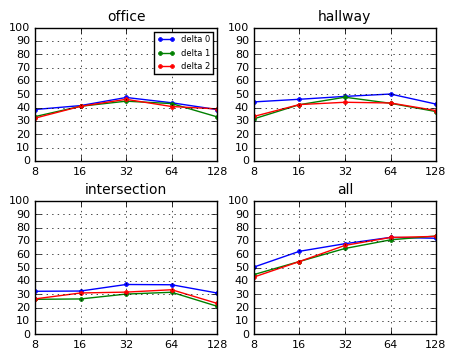
\includegraphics{chapters/results-identify-ssfgmm/r-095}
    \label{fig:r-095}
\end{figure}

\newpage
\section{Table and curves for $r = 0.99$}

\begin{table}[h]
    \centering
    \begin{tabular}{|c|c|M{2cm}|M{2cm}|M{2cm}|M{2cm}|}
    \hline
    $\boldsymbol{\Delta}$ & \bf{M} & \bf{Office} & \bf{Hallway} & \bf{Intersection} & \bf{All} \\ \hline \hline & \bf{8} & 41.55 & 51.31 & 41.13 & 63.70 \\ \cline{2-6} & \bf{16} & 47.42 & 56.13 & 45.10 & 71.64 \\ \cline{2-6}
    \multirow{5}*\bf{\textbf 0} & \bf{32} & 48.73 & 56.98 & 43.83 & 78.32 \\ \cline{2-6} & \bf{64} & 49.61 & 55.52 & 43.21 & 80.83 \\ \cline{2-6} & \bf{128} & 47.15 & 50.69 & 38.93 & 81.13 \\ \hline \hline & \bf{8} & 43.90 & 52.16 & 43.09 & 65.90 \\ \cline{2-6} & \bf{16} & 49.31 & 58.68 & 47.22 & 76.85 \\ \cline{2-6}
    \multirow{5}*\bf{\textbf 1} & \bf{32} & 52.16 & 60.42 & 48.73 & 83.37 \\ \cline{2-6} & \bf{64} & 53.94 & 60.03 & 48.77 & 86.03 \\ \cline{2-6} & \bf{128} & 49.88 & 54.63 & 45.83 & 87.15 \\ \hline \hline & \bf{8} & 43.87 & 55.25 & 43.94 & 66.63 \\ \cline{2-6} & \bf{16} & 49.65 & 60.61 & 48.11 & 77.97 \\ \cline{2-6}
    \multirow{5}*\bf{\textbf 2} & \bf{32} & 53.28 & 62.77 & 52.20 & 84.14 \\ \cline{2-6} & \bf{64} & 53.40 & 61.11 & 51.93 & 88.31 \\ \cline{2-6} & \bf{128} & 50.23 & 54.17 & 46.03 & 88.43 \\ \hline
    \end{tabular}
    \caption{Speaker identification success rates and $r = 0.99$.}
    \label{tab:identify_speakers_0.99}
\end{table}


\begin{figure}[ht]
    \centering
    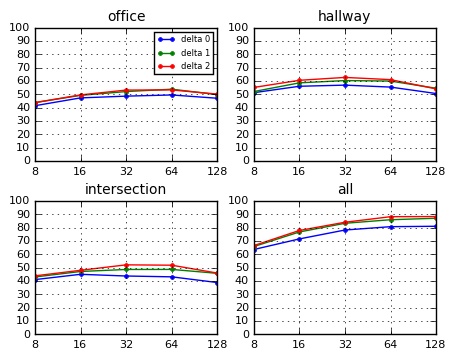
\includegraphics{chapters/results-identify-ssfgmm/r-099}
    \label{fig:r-099}
\end{figure}

\newpage
\section{Table and curves for $r = 1$}

\begin{table}[h]
    \centering
    \begin{tabular}{|c|c|M{2cm}|M{2cm}|M{2cm}|M{2cm}|}
    \hline
    $\boldsymbol{\Delta}$ & \bf{M} & \bf{Office} & \bf{Hallway} & \bf{Intersection} & \bf{All} \\
    \hline
    \hline
     & \bf{8} & 40.86 & 52.01 & 41.32 & 64.47 \\
    \cline{2-6}
     & \bf{16} & 47.69 & 56.52 & 44.79 & 72.22 \\
    \cline{2-6}
    \multirow{5}{*}\bf{\textbf 0} & \bf{32} & 49.50 & 57.72 & 47.61 & 77.74 \\
    \cline{2-6}
     & \bf{64} & 50.00 & 57.95 & 45.68 & 81.25 \\
    \cline{2-6}
     & \bf{128} & 48.65 & 53.43 & 42.63 & 81.67 \\
    \hline
    \hline
     & \bf{8} & 44.25 & 53.97 & 45.60 & 66.94 \\
    \cline{2-6}
     & \bf{16} & 50.42 & 62.00 & 50.54 & 78.24 \\
    \cline{2-6}
    \multirow{5}{*}\bf{\textbf 1} & \bf{32} & 54.28 & 63.54 & 53.86 & 84.45 \\
    \cline{2-6}
     & \bf{64} & 55.09 & 64.81 & 52.85 & 87.31 \\
    \cline{2-6}
     & \bf{128} & 53.32 & 59.99 & 50.46 & 88.85 \\
    \hline
    \hline
     & \bf{8} & 44.37 & 57.06 & 47.30 & 69.64 \\
    \cline{2-6}
     & \bf{16} & 50.89 & 62.81 & 52.12 & 78.78 \\
    \cline{2-6}
    \multirow{5}{*}\bf{\textbf 2} & \bf{32} & 54.90 & 65.01 & 56.29 & 86.00 \\
    \cline{2-6}
     & \bf{64} & 56.06 & 64.70 & 56.56 & 89.16 \\
    \cline{2-6}
     & \bf{128} & 52.55 & 60.73 & 49.58 & 90.66 \\
    \hline
    \end{tabular}
    \caption{Identification rates for enrolled speakers with $r = 1.00$.}
    \label{tab:identify_speakers_1.00}
\end{table}


\begin{figure}[ht]
    \centering
    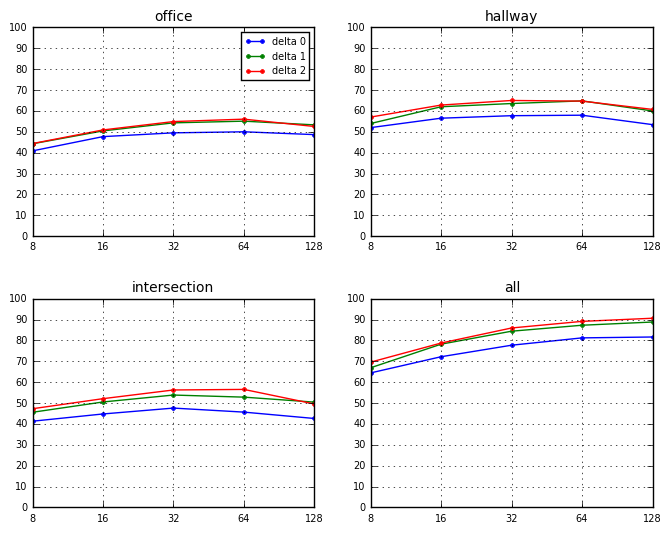
\includegraphics{chapters/results-identify-ssfgmm/r-100}
    \label{fig:r-100}
\end{figure}

\newpage
\section{Table and curves for $r = 1.01$}

\begin{table}[h]
    \centering
    \begin{tabular}{|c|c|M{2cm}|M{2cm}|M{2cm}|M{2cm}|}
    \hline
    $\boldsymbol{\Delta}$ & \bf{M} & \bf{Office} & \bf{Hallway} & \bf{Intersection} & \bf{All} \\ \hline \hline & \bf{8} & 40.16 & 52.51 & 43.02 & 61.69 \\ \cline{2-6} & \bf{16} & 46.88 & 57.10 & 47.80 & 71.84 \\ \cline{2-6}
    \multirow{5}*\bf{\textbf 0} & \bf{32} & 49.92 & 59.30 & 49.11 & 76.66 \\ \cline{2-6} & \bf{64} & 50.19 & 58.95 & 48.92 & 79.94 \\ \cline{2-6} & \bf{128} & 48.38 & 55.56 & 45.22 & 81.52 \\ \hline \hline & \bf{8} & 43.36 & 54.90 & 45.18 & 65.28 \\ \cline{2-6} & \bf{16} & 49.58 & 61.07 & 53.74 & 76.74 \\ \cline{2-6}
    \multirow{5}*\bf{\textbf 1} & \bf{32} & 55.02 & 66.44 & 56.64 & 83.60 \\ \cline{2-6} & \bf{64} & 56.02 & 66.28 & 56.25 & 88.00 \\ \cline{2-6} & \bf{128} & 55.17 & 62.23 & 54.32 & 89.51 \\ \hline \hline & \bf{8} & 45.10 & 53.74 & 47.22 & 66.44 \\ \cline{2-6} & \bf{16} & 50.81 & 64.31 & 53.59 & 78.05 \\ \cline{2-6}
    \multirow{5}*\bf{\textbf 2} & \bf{32} & 56.56 & 67.09 & 58.49 & 84.72 \\ \cline{2-6} & \bf{64} & 56.10 & 66.90 & 58.33 & 89.74 \\ \cline{2-6} & \bf{128} & 55.02 & 63.54 & 56.33 & 90.55 \\ \hline
    \end{tabular}
    \label{tab:identify_speakers_1.01}
\end{table}


\begin{figure}[ht]
    \centering
    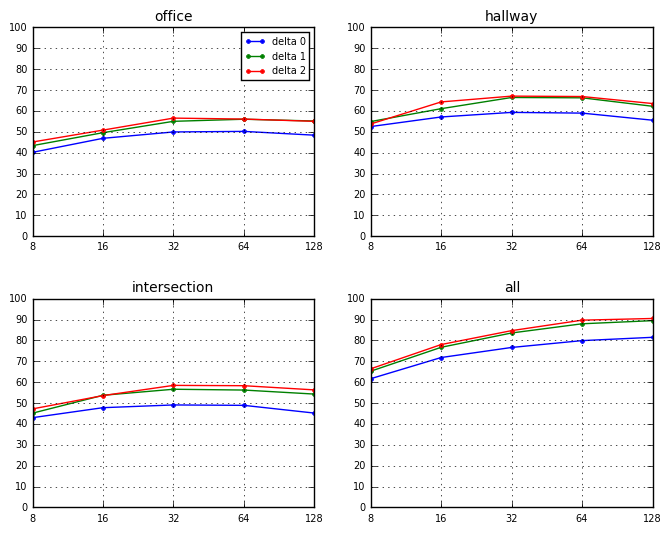
\includegraphics{chapters/results-identify-ssfgmm/r-101}
    \label{fig:r-101}
\end{figure}

\newpage
\section{Table and curves for $r = 1.05$}

\begin{table}[h]
    \centering
    \begin{tabular}{|c|c|M{2cm}|M{2cm}|M{2cm}|M{2cm}|}
    \hline
    $\boldsymbol{\Delta}$ & \bf{M} & \bf{Office} & \bf{Hallway} & \bf{Intersection} & \bf{All} \\ \hline \hline & \bf{8} & 22.22 & 33.02 & 34.80 & 30.71 \\ \cline{2-6} & \bf{16} & 32.52 & 41.32 & 42.67 & 42.32 \\ \cline{2-6}
    \multirow{5}*\bf{\textbf 0} & \bf{32} & 40.78 & 51.20 & 48.92 & 52.70 \\ \cline{2-6} & \bf{64} & 46.68 & 56.56 & 53.51 & 62.19 \\ \cline{2-6} & \bf{128} & 49.15 & 59.57 & 55.13 & 69.91 \\ \hline \hline & \bf{8} & 18.56 & 23.88 & 26.97 & 22.15 \\ \cline{2-6} & \bf{16} & 28.20 & 39.00 & 39.78 & 32.87 \\ \cline{2-6}
    \multirow{5}*\bf{\textbf 1} & \bf{32} & 38.39 & 51.58 & 50.46 & 50.08 \\ \cline{2-6} & \bf{64} & 49.11 & 63.46 & 58.33 & 62.96 \\ \cline{2-6} & \bf{128} & 57.99 & 66.32 & 59.41 & 75.96 \\ \hline \hline & \bf{8} & 17.52 & 25.15 & 28.43 & 19.41 \\ \cline{2-6} & \bf{16} & 28.94 & 38.27 & 42.44 & 34.30 \\ \cline{2-6}
    \multirow{5}*\bf{\textbf 2} & \bf{32} & 40.74 & 50.31 & 49.38 & 49.88 \\ \cline{2-6} & \bf{64} & 50.42 & 61.23 & 58.87 & 63.77 \\ \cline{2-6} & \bf{128} & 57.68 & 67.52 & 62.00 & 77.55 \\ \hline
    \end{tabular}
    \caption{Speaker identification success rates and $r = 1.05$.}
    \label{tab:identify_speakers_1.05}
\end{table}


\begin{figure}[ht]
    \centering
    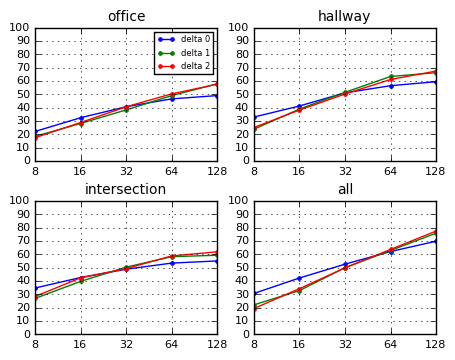
\includegraphics{chapters/results-identify-ssfgmm/r-105}
    \label{fig:r-105}
\end{figure}

\chapter{Verification}
\label{apx:results-verify}

\begin{table}[h]
    \centering
    \begin{tabular}{|c|c|M{2cm}|M{2cm}|M{2cm}|M{2cm}|}
    \hline
    $\boldsymbol{\Delta}$ & \bf{M} & \bf{Office} & \bf{Hallway} & \bf{Intersection} & \bf{All} \\
    \hline
    \hline
     & \bf{8} & 22.88 & 19.06 & 22.30 & 14.81 \\
    \cline{2-6}
     & \bf{16} & 21.49 & 16.71 & 21.49 & 11.19 \\
    \cline{2-6}
    \multirow{5}{*}\bf{\textbf 0} & \bf{32} & 21.14 & 16.05 & 20.94 & 9.61 \\
    \cline{2-6}
     & \bf{64} & 21.18 & 16.98 & 21.34 & 8.87 \\
    \cline{2-6}
     & \bf{128} & 21.49 & 19.33 & 23.74 & 8.60 \\
    \hline
    \hline
     & \bf{8} & 23.15 & 17.67 & 21.34 & 13.93 \\
    \cline{2-6}
     & \bf{16} & 20.80 & 15.78 & 18.33 & 10.07 \\
    \cline{2-6}
    \multirow{5}{*}\bf{\textbf 1} & \bf{32} & 19.06 & 15.31 & 18.45 & 7.87 \\
    \cline{2-6}
     & \bf{64} & 19.02 & 15.28 & 18.87 & 6.72 \\
    \cline{2-6}
     & \bf{128} & 20.14 & 17.79 & 20.37 & 6.79 \\
    \hline
    \hline
     & \bf{8} & 22.42 & 17.52 & 22.03 & 13.92 \\
    \cline{2-6}
     & \bf{16} & 20.22 & 15.32 & 18.20 & 10.06 \\
    \cline{2-6}
    \multirow{5}{*}\bf{\textbf 2} & \bf{32} & 19.48 & 15.20 & 17.36 & 7.75 \\
    \cline{2-6}
     & \bf{64} & 18.67 & 15.82 & 18.48 & 6.25 \\
    \cline{2-6}
     & \bf{128} & 19.80 & 17.94 & 21.26 & 6.40 \\
    \hline
    \end{tabular}
\end{table}


\begin{figure}[ht]
	\centering
	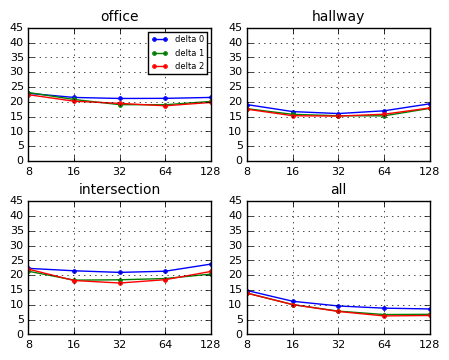
\includegraphics{chapters/results-verify/speakers/eer}
	\caption{Verification EERs for enrolled speakers.}
	\label{fig:results-verify}
\end{figure}

\begin{figure}[ht]
	\centering
	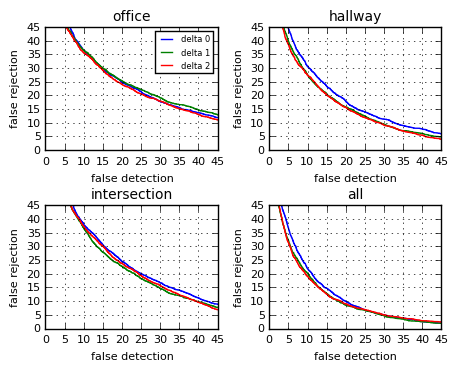
\includegraphics{chapters/results-verify/speakers/det_M_8}
	\caption{DET Curves with $M = 8$, for enrolled speakers.}
	\label{fig:results-verify-M_8}
\end{figure}

\begin{figure}[ht]
	\centering
	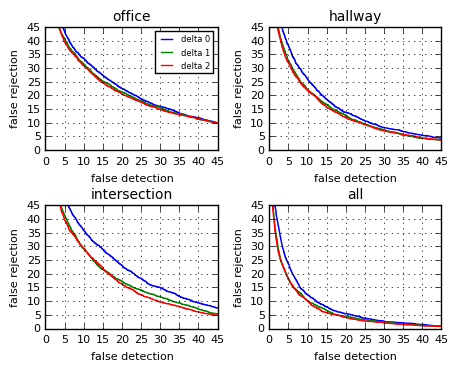
\includegraphics{chapters/results-verify/speakers/det_M_16}
	\caption{DET Curves with $M = 16$, for enrolled speakers.}
	\label{fig:results-verify-M_16}
\end{figure}

\begin{figure}[ht]
	\centering
	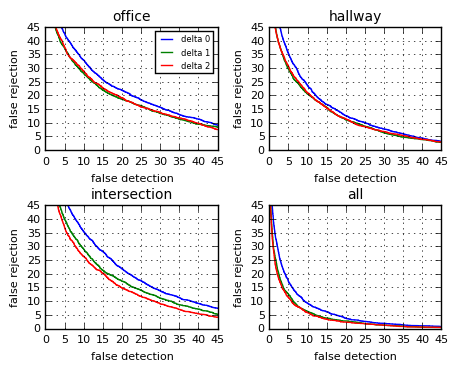
\includegraphics{chapters/results-verify/speakers/det_M_32}
	\caption{DET Curves with $M = 32$, for enrolled speakers.}
	\label{fig:results-verify-M_32}
\end{figure}

\begin{figure}[ht]
	\centering
	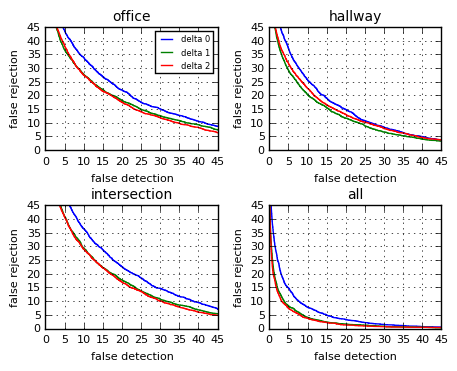
\includegraphics{chapters/results-verify/speakers/det_M_64}
	\caption{DET Curves with $M = 64$, for enrolled speakers.}
	\label{fig:results-verify-M_64}
\end{figure}

\clearpage
\begin{figure}[ht]
	\centering
	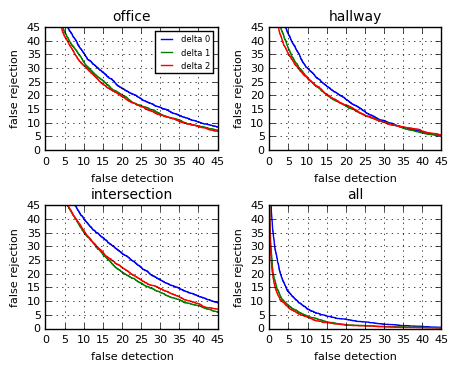
\includegraphics{chapters/results-verify/speakers/det_M_128}
	\caption{DET Curves with $M = 128$, for enrolled speakers.}
	\label{fig:results-verify-M_128}
\end{figure}

\newpage
\begin{table}[h]
    \centering
    \begin{tabular}{|c|c|M{2cm}|M{2cm}|M{2cm}|M{2cm}|}
    \hline
    $\boldsymbol{\Delta}$ & \bf{M} & \bf{Office} & \bf{Hallway} & \bf{Intersection} & \bf{All} \\ 
    \hline 
    \hline
     & \bf{8} & 25.38 & 21.00 & 23.66 & 18.21 \\
    \cline{2-6}
     & \bf{16} & 23.14 & 18.40 & 21.49 & 14.39 \\
    \cline{2-6}
    \multirow{5}{*}\bf{\textbf 0} & \bf{32} & 21.71 & 17.13 & 20.99 & 12.93 \\
    \cline{2-6}
     & \bf{64} & 20.64 & 16.55 & 19.98 & 11.61 \\
    \cline{2-6}
     & \bf{128} & 19.79 & 15.82 & 20.07 & 11.29 \\
    \hline
    \hline
     & \bf{8} & 25.31 & 21.83 & 24.73 & 18.59 \\
    \cline{2-6}
     & \bf{16} & 22.61 & 17.52 & 20.80 & 14.20 \\
    \cline{2-6}
    \multirow{5}{*}\bf{\textbf 1} & \bf{32} & 21.07 & 16.28 & 19.52 & 11.30 \\
    \cline{2-6}
     & \bf{64} & 18.90 & 14.51 & 17.44 & 9.58 \\
    \cline{2-6}
     & \bf{128} & 17.44 & 13.46 & 16.62 & 7.80 \\
    \hline
    \hline
     & \bf{8} & 24.11 & 21.13 & 22.68 & 18.87 \\
    \cline{2-6}
     & \bf{16} & 21.99 & 17.63 & 19.47 & 13.59 \\
    \cline{2-6}
    \multirow{5}{*}\bf{\textbf 2} & \bf{32} & 20.29 & 15.51 & 17.67 & 10.57 \\
    \cline{2-6}
     & \bf{64} & 18.71 & 13.77 & 17.01 & 8.91 \\
    \cline{2-6}
     & \bf{128} & 17.48 & 12.43 & 15.97 & 7.56 \\
    \hline
    \end{tabular}
    \caption{Verification EERs for enrolled speakers for adaptations = m.}
    \label{tab:verify_adapted_m}
\end{table}


\begin{figure}[ht]
	\centering
	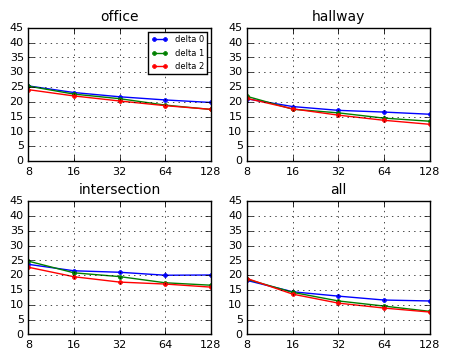
\includegraphics{chapters/results-verify/adapted_m/eer}
	\caption{Verification EERs for enrolled speakers with adaptations = m.}
	\label{fig:results-verify-adapted_m}
\end{figure}

\begin{figure}[ht]
	\centering
	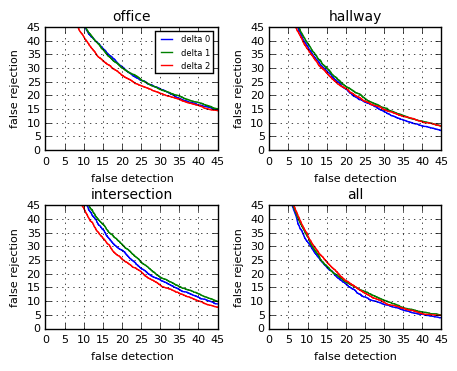
\includegraphics{chapters/results-verify/adapted_m/det_M_8}
	\caption{DET Curves with $M = 8$, for enrolled speakers with adaptations = m.}
	\label{fig:results-verify-adapted_m-M_8}
\end{figure}

\begin{figure}[ht]
	\centering
	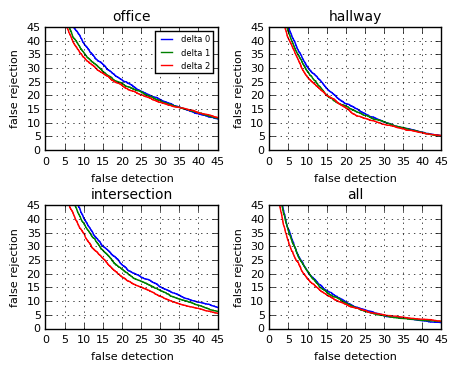
\includegraphics{chapters/results-verify/adapted_m/det_M_16}
	\caption{DET Curves with $M = 16$, for enrolled speakers with adaptations = m.}
	\label{fig:results-verify-adapted_m-M_16}
\end{figure}

\begin{figure}[ht]
	\centering
	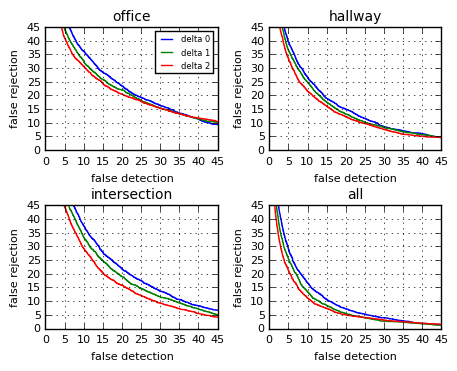
\includegraphics{chapters/results-verify/adapted_m/det_M_32}
	\caption{DET Curves with $M = 32$, for enrolled speakers with adaptations = m.}
	\label{fig:results-verify-adapted_m-M_32}
\end{figure}

\begin{figure}[ht]
	\centering
	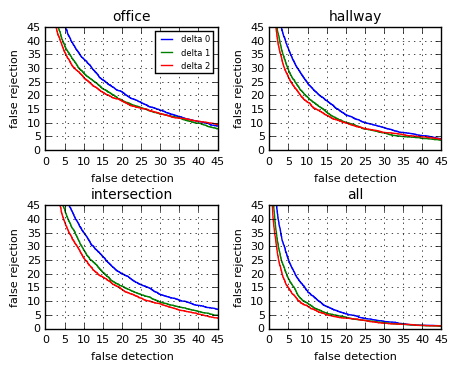
\includegraphics{chapters/results-verify/adapted_m/det_M_64}
	\caption{DET Curves with $M = 64$, for enrolled speakers with adaptations = m.}
	\label{fig:results-verify-adapted_m-M_64}
\end{figure}

\clearpage
\begin{figure}[ht]
	\centering
	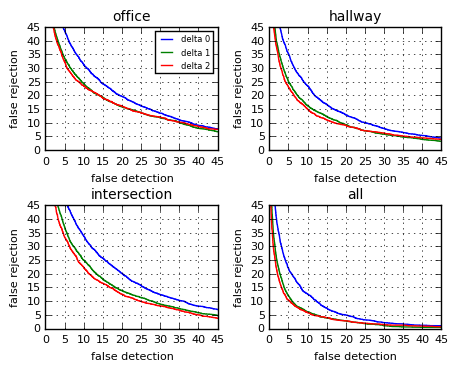
\includegraphics{chapters/results-verify/adapted_m/det_M_128}
	\caption{DET Curves with $M = 128$, for enrolled speakers with adaptations = m.}
	\label{fig:results-verify-adapted_m-M_128}
\end{figure}

\newpage
\begin{table}[h]
    \centering
    \begin{tabular}{|c|c|M{2cm}|M{2cm}|M{2cm}|M{2cm}|}
    \hline
    $\boldsymbol{\Delta}$ & \bf{M} & \bf{Office} & \bf{Hallway} & \bf{Intersection} & \bf{All} \\ 
    \hline 
    \hline
     & \bf{8} & 23.68 & 19.32 & 23.84 & 16.09 \\
    \cline{2-6}
     & \bf{16} & 21.57 & 17.71 & 22.96 & 13.46 \\
    \cline{2-6}
    \multirow{5}{*}\bf{\textbf 0} & \bf{32} & 20.72 & 16.48 & 23.38 & 11.42 \\
    \cline{2-6}
     & \bf{64} & 20.52 & 18.51 & 24.16 & 11.07 \\
    \cline{2-6}
     & \bf{128} & 21.95 & 19.96 & 26.04 & 10.72 \\
    \hline
    \hline
     & \bf{8} & 23.42 & 19.33 & 23.45 & 15.39 \\
    \cline{2-6}
     & \bf{16} & 21.26 & 16.24 & 20.76 & 12.19 \\
    \cline{2-6}
    \multirow{5}{*}\bf{\textbf 1} & \bf{32} & 19.56 & 15.50 & 19.98 & 9.72 \\
    \cline{2-6}
     & \bf{64} & 18.22 & 15.24 & 20.33 & 8.22 \\
    \cline{2-6}
     & \bf{128} & 17.52 & 15.69 & 20.56 & 7.75 \\
    \hline
    \hline
     & \bf{8} & 22.49 & 18.40 & 22.49 & 14.62 \\
    \cline{2-6}
     & \bf{16} & 20.87 & 16.24 & 19.99 & 11.56 \\
    \cline{2-6}
    \multirow{5}{*}\bf{\textbf 2} & \bf{32} & 19.48 & 14.93 & 18.75 & 9.30 \\
    \cline{2-6}
     & \bf{64} & 19.25 & 15.36 & 19.02 & 7.94 \\
    \cline{2-6}
     & \bf{128} & 19.29 & 16.55 & 19.28 & 7.25 \\
    \hline
    \end{tabular}
    \caption{Verification EERs for enrolled speakers for adaptations = mv.}
    \label{tab:verify_adapted_mv}
\end{table}


\begin{figure}[ht]
	\centering
	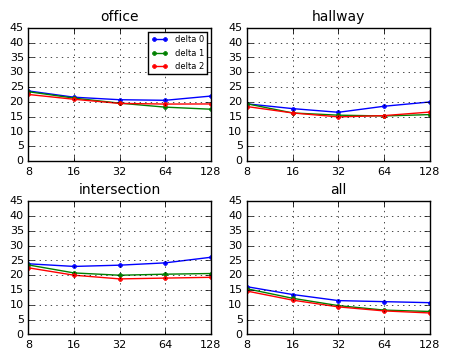
\includegraphics{chapters/results-verify/adapted_mv/eer}
	\caption{Verification EERs for enrolled speakers with adaptations = mv.}
	\label{fig:results-verify-adapted_mv}
\end{figure}

\begin{figure}[ht]
	\centering
	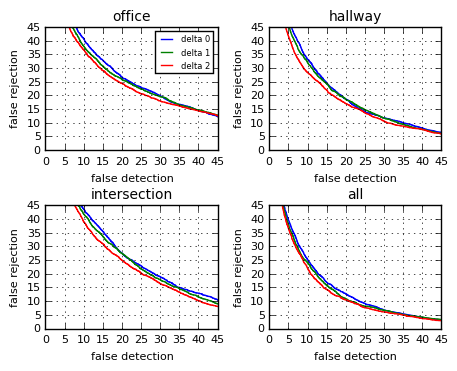
\includegraphics{chapters/results-verify/adapted_mv/det_M_8}
	\caption{DET Curves with $M = 8$, for enrolled speakers with adaptations = mv.}
	\label{fig:results-verify-adapted_mv-M_8}
\end{figure}

\begin{figure}[ht]
	\centering
	\includegraphics{chapters/results-verify/adapted_mv/det_M_16}
	\caption{DET Curves with $M = 16$, for enrolled speakers with adaptations = mv.}
	\label{fig:results-verify-adapted_mv-M_16}
\end{figure}

\begin{figure}[ht]
	\centering
	\includegraphics{chapters/results-verify/adapted_mv/det_M_32}
	\caption{DET Curves with $M = 32$, for enrolled speakers with adaptations = mv.}
	\label{fig:results-verify-adapted_mv-M_32}
\end{figure}

\begin{figure}[ht]
	\centering
	\includegraphics{chapters/results-verify/adapted_mv/det_M_64}
	\caption{DET Curves with $M = 64$, for enrolled speakers with adaptations = mv.}
	\label{fig:results-verify-adapted_mv-M_64}
\end{figure}

\clearpage
\begin{figure}[ht]
	\centering
	\includegraphics{chapters/results-verify/adapted_mv/det_M_128}
	\caption{DET Curves with $M = 128$, for enrolled speakers with adaptations = mv.}
	\label{fig:results-verify-adapted_mv-M_128}
\end{figure}

\newpage
\begin{table}[h]
    \centering
    \begin{tabular}{|c|c|M{2cm}|M{2cm}|M{2cm}|M{2cm}|}
    \hline
    $\boldsymbol{\Delta}$ & \bf{M} & \bf{Office} & \bf{Hallway} & \bf{Intersection} & \bf{All} \\ 
    \hline 
    \hline
     & \bf{8} & 25.58 & 21.17 & 23.68 & 18.21 \\
    \cline{2-6}
     & \bf{16} & 23.23 & 18.09 & 21.83 & 14.74 \\
    \cline{2-6}
    \multirow{5}{*}\bf{\textbf 0} & \bf{32} & 21.84 & 16.82 & 21.03 & 12.73 \\
    \cline{2-6}
     & \bf{64} & 20.56 & 16.20 & 19.78 & 11.23 \\
    \cline{2-6}
     & \bf{128} & 19.95 & 15.28 & 19.14 & 10.84 \\
    \hline
    \hline
     & \bf{8} & 25.54 & 21.60 & 24.88 & 18.36 \\
    \cline{2-6}
     & \bf{16} & 22.84 & 17.32 & 21.07 & 14.35 \\
    \cline{2-6}
    \multirow{5}{*}\bf{\textbf 1} & \bf{32} & 21.14 & 16.09 & 19.52 & 11.42 \\
    \cline{2-6}
     & \bf{64} & 19.52 & 14.40 & 17.71 & 9.53 \\
    \cline{2-6}
     & \bf{128} & 17.90 & 13.19 & 16.47 & 7.84 \\
    \hline
    \hline
     & \bf{8} & 24.27 & 20.76 & 22.61 & 18.56 \\
    \cline{2-6}
     & \bf{16} & 22.18 & 16.98 & 19.68 & 13.62 \\
    \cline{2-6}
    \multirow{5}{*}\bf{\textbf 2} & \bf{32} & 20.22 & 15.36 & 17.64 & 10.49 \\
    \cline{2-6}
     & \bf{64} & 18.72 & 13.47 & 16.95 & 8.96 \\
    \cline{2-6}
     & \bf{128} & 17.55 & 12.46 & 15.74 & 7.52 \\
    \hline
    \end{tabular}
    \caption{Verification EERs for enrolled speakers for adaptations = wm.}
    \label{tab:verify_adapted_wm}
\end{table}


\begin{figure}[ht]
	\centering
	\includegraphics{chapters/results-verify/adapted_wm/eer}
	\caption{Verification EERs for enrolled speakers with adaptations = wm.}
	\label{fig:results-verify-adapted_wm}
\end{figure}

\begin{figure}[ht]
	\centering
	\includegraphics{chapters/results-verify/adapted_wm/det_M_8}
	\caption{DET Curves with $M = 8$, for enrolled speakers with adaptations = wm.}
	\label{fig:results-verify-adapted_wm-M_8}
\end{figure}

\begin{figure}[ht]
	\centering
	\includegraphics{chapters/results-verify/adapted_wm/det_M_16}
	\caption{DET Curves with $M = 16$, for enrolled speakers with adaptations = wm.}
	\label{fig:results-verify-adapted_wm-M_16}
\end{figure}

\begin{figure}[ht]
	\centering
	\includegraphics{chapters/results-verify/adapted_wm/det_M_32}
	\caption{DET Curves with $M = 32$, for enrolled speakers with adaptations = wm.}
	\label{fig:results-verify-adapted_wm-M_32}
\end{figure}

\begin{figure}[ht]
	\centering
	\includegraphics{chapters/results-verify/adapted_wm/det_M_64}
	\caption{DET Curves with $M = 64$, for enrolled speakers with adaptations = wm.}
	\label{fig:results-verify-adapted_wm-M_64}
\end{figure}

\clearpage
\begin{figure}[ht]
	\centering
	\includegraphics{chapters/results-verify/adapted_wm/det_M_128}
	\caption{DET Curves with $M = 128$, for enrolled speakers with adaptations = wm.}
	\label{fig:results-verify-adapted_wm-M_128}
\end{figure}

\newpage
\begin{table}[h]
    \centering
    \begin{tabular}{|c|c|M{2cm}|M{2cm}|M{2cm}|M{2cm}|}
    \hline
    $\boldsymbol{\Delta}$ & \bf{M} & \bf{Office} & \bf{Hallway} & \bf{Intersection} & \bf{All} \\ 
    \hline 
    \hline
     & \bf{8} & 23.96 & 19.49 & 23.84 & 16.04 \\
    \cline{2-6}
     & \bf{16} & 21.92 & 17.33 & 22.64 & 13.50 \\
    \cline{2-6}
    \multirow{5}{*}\bf{\textbf 0} & \bf{32} & 20.87 & 16.51 & 22.88 & 11.69 \\
    \cline{2-6}
     & \bf{64} & 20.41 & 17.51 & 23.23 & 11.07 \\
    \cline{2-6}
     & \bf{128} & 20.84 & 18.06 & 23.92 & 10.30 \\
    \hline
    \hline
     & \bf{8} & 23.35 & 19.06 & 23.58 & 15.51 \\
    \cline{2-6}
     & \bf{16} & 21.76 & 16.16 & 20.76 & 12.35 \\
    \cline{2-6}
    \multirow{5}{*}\bf{\textbf 1} & \bf{32} & 19.64 & 15.47 & 19.98 & 9.99 \\
    \cline{2-6}
     & \bf{64} & 18.44 & 15.16 & 19.98 & 8.49 \\
    \cline{2-6}
     & \bf{128} & 17.55 & 15.01 & 19.68 & 7.80 \\
    \hline
    \hline
     & \bf{8} & 22.65 & 18.36 & 22.38 & 14.78 \\
    \cline{2-6}
     & \bf{16} & 21.03 & 16.06 & 19.99 & 11.77 \\
    \cline{2-6}
    \multirow{5}{*}\bf{\textbf 2} & \bf{32} & 19.71 & 14.67 & 18.44 & 9.44 \\
    \cline{2-6}
     & \bf{64} & 19.14 & 15.01 & 18.49 & 7.99 \\
    \cline{2-6}
     & \bf{128} & 18.94 & 15.78 & 18.71 & 7.37 \\
    \hline
    \end{tabular}
    \caption{Verification EERs for enrolled speakers for adaptations = wmv.}
    \label{tab:verify_adapted_wmv}
\end{table}


\begin{figure}[ht]
	\centering
	\includegraphics{chapters/results-verify/adapted_wmv/eer}
	\caption{Verification EERs for enrolled speakers with adaptations = wmv.}
	\label{fig:results-verify-adapted_wmv}
\end{figure}

\begin{figure}[ht]
	\centering
	\includegraphics{chapters/results-verify/adapted_wmv/det_M_8}
	\caption{DET Curves with $M = 8$, for enrolled speakers with adaptations = wmv.}
	\label{fig:results-verify-adapted_wmv-M_8}
\end{figure}

\begin{figure}[ht]
	\centering
	\includegraphics{chapters/results-verify/adapted_wmv/det_M_16}
	\caption{DET Curves with $M = 16$, for enrolled speakers with adaptations = wmv.}
	\label{fig:results-verify-adapted_wmv-M_16}
\end{figure}

\begin{figure}[ht]
	\centering
	\includegraphics{chapters/results-verify/adapted_wmv/det_M_32}
	\caption{DET Curves with $M = 32$, for enrolled speakers with adaptations = wmv.}
	\label{fig:results-verify-adapted_wmv-M_32}
\end{figure}

\begin{figure}[ht]
	\centering
	\includegraphics{chapters/results-verify/adapted_wmv/det_M_64}
	\caption{DET Curves with $M = 64$, for enrolled speakers with adaptations = wmv.}
	\label{fig:results-verify-adapted_wmv-M_64}
\end{figure}

\clearpage
\begin{figure}[ht]
	\centering
	\includegraphics{chapters/results-verify/adapted_wmv/det_M_128}
	\caption{DET Curves with $M = 128$, for enrolled speakers with adaptations = wmv.}
	\label{fig:results-verify-adapted_wmv-M_128}
\end{figure}


\printbibliography

\end{document}